% === Revtex Declaration ===
\documentclass[aps, 10pt, english, twoside, pra, nofootinbib, tightenlines, longbibliography, superscriptaddress]{revtex4-1}

% === All of the Packages I use frequently ===
\usepackage{../../packages/document_config}
\usepackage{../../packages/shared}
\usepackage{../../packages/misc_commands}

\renewcommand{\Events}[1]{\mathcal{S}\br{#1}} % This notation is conflicting

% === Causal structure formatting for tikz ===
% =========================
% Causal Structure Diagrams
% =========================
\definecolor{obs_outline}{RGB}{51,157,215}
\definecolor{obs_fill}{RGB}{222,253,255}
\definecolor{obs_text}{RGB}{0,0,0}
\definecolor{lat_outline}{RGB}{251,141,54}
\definecolor{cause}{RGB}{30, 0, 30}
\definecolor{lat_fill}{RGB}{255,213,153}
\definecolor{lat_text}{RGB}{0,0,0}
\tikzset{square/.style={regular polygon,regular polygon sides=4}}
\tikzset{triangle/.style={regular polygon,regular polygon sides=3}}
\tikzset{observed/.style={obs_text, align=center, triangle, thick, draw=obs_outline, fill=obs_fill, inner sep=-0.2em, text width=1.5em}}
\tikzset{latent/.style={lat_text, align=center, circle, thick, draw=lat_outline, fill=lat_fill, text width=1.5em, inner sep=0.2em}}
\tikzset{fade/.style={opacity=0.2}}
\tikzset{unfade/.style={opacity=1.0}}
% TikZ stile to apply keys only on specific beamer overlays
% onslide=<overlay spec>{key=value, key=value, ...}
\tikzset{onslide/.code args={<#1>#2}{%
  \only<#1>{\pgfkeysalso{#2}}%
}}
\providecommand{\p}[1]{#1}
% \tikzset{cause/.style={mid arrow/.style={postaction={decorate,decoration={markings, mark=at position .5 with {\arrow[#1]{stealth}}}}},}}
\tikzset{
    % style to apply some styles to each segment of a path
    on each segment/.style={
        decorate,
        decoration={
            show path construction,
            moveto code={},
            lineto code={
                \path [#1]
                (\tikzinputsegmentfirst) -- (\tikzinputsegmentlast);
            },
            curveto code={
                \path [#1] (\tikzinputsegmentfirst)
                .. controls
                (\tikzinputsegmentsupporta) and (\tikzinputsegmentsupportb)
                ..
                (\tikzinputsegmentlast);
            },
            closepath code={
                \path [#1]
                (\tikzinputsegmentfirst) -- (\tikzinputsegmentlast);
            },
        },
    },
    % style to add an arrow in the middle of a path
    mid arrow/.style={postaction={decorate,decoration={
                markings,
                mark=at position .6 with {\arrow[scale=1.5, cause]{stealth}}
            }}},
}
% =========================
% =========================

\begin{document}
    \title{Causal Compatibility Inequalities Admitting of Quantum Violations in the Triangle Structure}
    \author{Thomas C. Fraser}
    \email{tcfraser@tcfraser.com}
    \affiliation{Perimeter Institute for Theoretical Physics, Waterloo, Ontario, Canada, N2L 2Y5}
    \affiliation{University of Waterloo, Waterloo, Ontario, Canada, N2L 3G1}
    \author{Elie Wolfe}
    \affiliation{Perimeter Institute for Theoretical Physics, Waterloo, Ontario, Canada, N2L 2Y5}
    % \email{ewolfe@perimeterinstitute.ca}
    \date{\today}
    \begin{abstract}
        It has long been recognized that certain quantum correlations are often incompatible with particular assumption about classical causal structure. Such correlations are sometimes termed non-local, although they are more accurately termed non-classical, as the presence of correlations certifies the genuinely non-classical nature of a causal setup in a device-independent fashion.  Whenever a quantum correlation violates a causal compatibility inequality (e.g. a Bell inequality) then the correlation is witnessed as non-classical. Any constraint which is satisfied by all correlations which \textit{are} classically compatible with a given causal structure defines a causal compatibility criterion. Such criteria were recently were recently derived for the Triangle structure [\href[pdfnewwindow]{http://arxiv.org/abs/1609.00672}{arXiv:1609.00672}] in the form of polynomial inequalities, begging the question: do any of those inequalities admit violation by quantum correlations? Numerical investigation suggests not, and we further conjecture that the set of correlations admitted by the classical Triangle structure is equivalent to the set of correlations admitted by its quantum generalization whenever the three observable variables are binary. Our main contribution in this work, however, is the derivation of new causal compatibility inequalities for the Triangle structure which \textit{do} admit quantum violation. We conclude by considering the possibility of quantum resources potentially qualitatively different from those known previously.
    \end{abstract}
    \maketitle
    \tableofcontents
    % \setlength{\parskip}{1em}

    \section{Introduction}
    \label{sec:introduction}
    In recent decades, the technical utility of quantum mechanics has become abundantly clear. In the realm of computation, quantum algorithms --- such as Shor's algorithm~\cite{Shor_1997} and numerous others~\cite{Jordan_2016} --- scale exponentially better than their classical counterparts. In the realm of secure communication, quantum protocols --- a popular example being Quantum Key Distribution~\cite{Bennett_2014} --- are able to provide privacy even against hypothetical adversaries with unlimited computational power, a desideratum which classical protocols are unable to fulfill. Throughout history, every aspect of quantum phenomena which fails to be emulated by classical resources has led to a practical exploitation of the non-classical feature in order to solve a some computational of communicational problem~\cite{Neilsen_Chaung_2011}. Motivated by past successes, a primal objective of modern quantum information theory is the discovery of new situations wherein quantum mechanics offers an advantage, and certification that the quantum advantage is genuine.

    From a foundational prospective, the most robust demonstrations of quantum phenomena with no classical emulation have involved Bell inequalities~\cite{Bell_1964}. Originally, Bell inequalities were derived as a way to show that no hidden variable theory could ever account for quantum mechanics; in this sense Bell inequalities are a response to the famous EPR paradox~\cite{EPR_Orig}. The enumeration of Bell inequalities has since become a widespread systematic way of demonstration the \textit{non-classicality} of a given observation. More recently it has been appreciated that Bell inequalities can understood as consequences of \term{causal inference}~\cite{Wood_2012}. Causal inference is concerned with classifying observations into those which can and cannot be explained by a hypothesized causal structure. The abstract nature of causal inference is responsible for its presence in numerous scientific fields including machine learning and biology~\cite{Pearl_2009,Pearl_2009_tr}. Causal compatibility inequalities, such as Bell and Instrumental inequalities, characterize the space of observations that are compatible with a hypothesized causal structure, albeit the characterization offered by practically derivable inequalities is often only an approximation. To derive the traditional Bell inequalities from causal inference one starts with a (classical) causal structure known as the Bell structure, as depicted in \cref{fig:bell_scenario}. The fundamental Bell structure involves non-communicating parties making measurements on some hidden shared resource $\la$, where the measurement outcomes ($A, B$) are presumed to be stochastic functions of the the local choices of measurement settings ($S_A, S_B$) and the shared resource $\la$. Quantum non-classicality in the Bell structure has been thoroughly studied since Bell's original work~\cite{Brunner_2013}. More complex structures, however, such as the correlation scenarios proposed by Fritz~\cite{Fritz_2012,Fritz_2014}, are much less understood. Here we investigate one particular causal structure: the Triangle structure (\cref{fig:triangle_structure}).

    The Triangle structure (\cref{fig:triangle_structure}) is a causal structure composed of $3$ parties labeled $A, B, C$ arranged in a triangular configuration while pair-wise sharing hidden/latent variables $X, Y, Z$. It has been extensively studied previously (see~\cite[Fig. 1]{Steudel_2010},~\cite[Fig. 6]{Chaves_2014},~\cite[Fig. 8]{Branciard_2012},~\cite[Fig. 8, App. E]{Henson_2014},~\cite[Fig. 3]{Fritz_2012},~\cite[Fig. 1]{Inflation}, $\ldots$). An overview of some milestone results is provided in \cref{sec:triangle_structure}. Identifying causal compatibility inequalities for this configuration has been seen as particularly challenging~\cite{Branciard_2012}. Further identifying causal compatibility inequalities of such high resolution that such inequalities can be violated by quantum-accessible distributions has remained out-of-reach for the Triangle structure.

    This work is the first, therefore, to find causal compatibility inequalities for the Triangle structure that are able to be violated by quantum-accessible distributions. This accomplishment was made possible through the combination of two previous developments. The first, an insight made by \citet{Fritz_2012} regarding the ability to re-interpret the Bell structure as a portion of the Triangle structure. The second, a new framework for solving causal inference problems developed by Wolfe \emph{et al.}~\cite{Inflation} called \term{The Inflation Technique}. Ultimately, this work serves as a validation that the Inflation Technique is sensitive enough to offer new insights into quantum non-classicality. Moreover, these new inequalities offer an avenue for recognizing previously unknown forms of non-classicality. The authors attempts to find such novel resources were met with only partial success, suggesting clear refinements for future exploration.

    The manuscript is organized into the following sections: \Cref{sec:causal_compatibility} recalls important notions from causal inference theory and sets up the notation to be used. \Cref{sec:bell_structure} offers a summary of the popular Bell structure and associated inequalities. \Cref{sec:triangle_structure} discusses the Triangle structure and provides an overview of existing research; identifying its stark differences from the Bell structure and motivating why the Triangle structure is worth studying. \Cref{sec:fritz_distribution} defines and discusses a singularly-quantum correlation first conceived of by \citet{Fritz_2012}, which we term the \term{Fritz distribution}. The Fritz distribution was proven to be non-classical without the use of inequalities --- this report fills in the desired missing inequalities. A sample of these inequalities are presented in \cref{sec:found_inequalities}, specifically \cref{eq:ww_ineq,eq:web_inequality,eq:symmetic_web_inequality}. Finally, \cref{sec:violations_noise} introduces a method for parameterizing the space of quantum-accessible distributions which we used to numerically optimize against our derived inequalities in search of stronger types of non-classicality. Additionally, the Fritz distribution is subjected to noise in order to measure the robustness of the derived inequalities. \Cref{sec:conclusions} concludes with proposed avenues for further research.

    \Cref{sec:inflation_technique} briefly summaries the Inflation Technique in the specific context of this work. Although the summary presented here is designed to be self-standing, a much more pedagogical introduction is offered by the original work~\cite{Inflation}. \Cref{sec:deriving_inequalities} demonstrates how the Inflation Technique was used to derive causal compatibility inequalities for the Triangle structure that are violated by quantum-accessible distributions.

    \section{Causal Compatibility}
    \label{sec:causal_compatibility}
    The task of causal inference is to determine the set of potentially observable probability distributions compatible with some hypothesis about causal relationships~\cite{Pearl_2009}. If an observed distribution can be explained by the hypothesized causal mechanism, then the distribution is said to be \textit{compatible} with said causal mechanism. In order to define compatibility rigorously, we first need to formally define the notion of a causal hypothesis.

    A hypothesis of causal mechanism is formally referred to as a \term{causal structure} and can be represented as a \term{directed acyclic graph}. A directed graph $\graph$ is an ordered tuple $\br{\nodes, \edges}$ of respectively \textit{nodes} and \textit{edges} where each edge $e \in \edges$ connects a \textit{pair} of nodes $n, m \in \nodes$ with a directed arrow $e = \bc{n \to m}$. A directed graph is \textit{acyclic} if there are no paths following the directions of the edges starting from and returning to the same node. The nodes $\nodes$ of a causal structure represent random variables while the edges $\edges$ represent a casual influence from one variable to another pursuant to the prescribed direction.

    Henceforth, we will utilize a number of familiar notions from graph theory and denote them accordingly. The \term{parents of a node} $n \in \nodes$ are all nodes which point directly into $n$, i.e. $\Pa[\graph]{n} \defined \bc{m \mid m \to n}$. Similarly defined are the \term{children of a node} $\Ch[\graph]{n} \defined \bc{m \mid n \to m}$. Recursively defined are the \term{ancestors of a node} $\An[\graph]{n} \defined \bigcup_{i\in\mathbb{N}} \Pa[\graph][i]{n}$ where $\Pa[\graph][i]{n} \defined \Pa[\graph]{\Pa[\graph][i-1]{n}}$ and $\Pa[\graph][0]{n} = n$ and the \term{descendants of a node} $\De[\graph]{n} \defined \bigcup_{i\in\mathbb{N}} \Ch[\graph][i]{n}$ where $\Ch[\graph][i]{n} \defined \Ch[\graph]{\Ch[\graph][i-1]{n}}$ and $\Ch[\graph][0]{n} = n$. Finally, we extend this notation to a subset of nodes $N \subseteq \nodes$ by performing a union over elements. As an example, the parents of the nodes $N \subseteq \nodes$ are denoted $\Pa[\graph]{N} = \bigcup_{n \in N} \Pa[\graph]{n}$.

    % A number of causal structures are depicted throughout this document (see \cref{fig:bell_scenario,fig:triangle_structure,fig:inflations}). As an example, the Triangle structure has $3$ observable nodes and $3$ latent nodes,
    % \[ \nodes_{O} = \bc{A, B, C} \qquad \nodes_{L} = \bc{X, Y, Z} \]
    % along with $6$ edges indicating that the latent nodes $\bc{X, Y, Z}$ cause and influence the observed nodes $\bc{A, B, C}$.
    % \[ \edges = \bc{\bc{X \to A}, \bc{Y \to A}, \bc{Y \to B}, \bc{Z \to B}, \bc{Z \to C}, \bc{X \to C}} \]

    Now that the notion of a causal structure $\graph$ is defined along with some standard graph-theoretic notation, it is now possible to precisely define the notion of compatibility between $\graph$ and a probability distribution $\prob[\nodes]$ defined over the nodes of $\graph$. Intuitively, the absence of certain causal connections within $\graph$ should limit the set of possible observations that can be made on $\graph$. Specifically, the causal structure $\graph$ hypothesizes that each variable $n \in \nodes$ is causally influenced by its parents $\Pa[\graph]{n}$, then $n$ should be independent of all other variables, except its own descendants when conditioned over $\Pa[\graph]{n}$. This is known as the \term{local Markov property}:\footnote{Here $A \indep B \mid C$ denotes statistical independence between $A$ and $B$ conditional on $C$ where $A,B,C \subseteq \nodes$, i.e. for a given probability distribution $\prob[\nodes]$, $\prob[AB \mid C] = \prob[A \mid C]\prob[B \mid C]$.}
    \[ n \indep \br{\nodes \setminus \De[\graph]{n}} \mid \Pa[\graph]{n} \quad \forall n \in \nodes \eq \label{eq:local_markov_property} \]
    If a given distribution $\prob[\nodes]$ defined over \textit{all} of the nodes $\nodes$ of $\graph$ satisfies \cref{eq:local_markov_property}, then $\prob[\nodes]$ is said to be \term{compatible with $\graph$}. Alternatively yet equivalently, the notion of compatibility can be interpreted as follows: a distribution $\prob[\nodes]$ is compatible with $\graph$ if $\prob[\nodes]$ can be consistently factorized into conditional probability distributions for each variable $n \in \nodes$ conditioned on its parents $\Pa[\graph]{n}$:
    \[ \prob[\nodes] = \prod_{n \in \nodes} \prob[n \mid \Pa[\graph]{n}] = \prob[n_1 \mid \Pa[\graph]{n_1}] \times \cdots \times \prob[n_k \mid \Pa[\graph]{n_k}] \eq \label{eq:compatibility_as_factorization}\]
    The conditional distributions in \cref{eq:compatibility_as_factorization} (i.e. $\{\prob[n \mid \Pa[\graph]{n}] \mid n \in \nodes\}$) are referred to as a set of \term{causal parameters for $\graph$}. If a distribution $\prob[\nodes]$ violates \cref{eq:local_markov_property} or equivalently cannot be factorized according to \cref{eq:compatibility_as_factorization}, $\prob[\nodes]$ is said to be \term{incompatible} with $\graph$. When one is specified with a joint distribution $\prob[\nodes]$ defined over all nodes of a causal structure $\graph$, it is trivially easy to verify whether or not $\prob[\nodes]$ is compatibility with $\graph$; \cref{sec:satisfaction_of_d_sep_relations} describes in detail how this is accomplished.

    A challenge is present when one is supplied with a partial observation, i.e. a joint distribution $\prob[\nodes_{O}]$ where $\nodes_{O} \subset \nodes$ is some subset of variables referred to as the \term{observable nodes} $\nodes_O$. In such cases, \cref{eq:compatibility_as_factorization} can not be verified by direction calculation because it is certainly possible that the parents of some observable node are themselves unobservable $\Pa[\graph]{\nodes_{O}} \not \subseteq \nodes_{O}$. In such cases, compatibility between $\graph$ and $\prob[\nodes_{O}]$ depends on the existence or non-existence of a set of causal parameters for $\graph$ such that $\prob[\nodes_{O}] = \prod_{n \in \nodes_{O}} \prob[n \mid \Pa[\graph]{n}]$. The unobservable nodes are termed \term{latent nodes} $\nodes_L = \nodes \setminus \nodes_{O}$ representing hidden random variables that are hidden either by some fundamental process or cannot be measured due to other limitations.
    \todo[TC]{Explain why this is difficult more.}
    \todo[TC]{Figure out if I should include d-sep here}
    \todo[TC]{Explain what this work and inflation accomplishes regarding this}

    In practice however, checking causal parameters systemically is intractable, especially when the cardinality (number of outcomes) of the latent variables is unspecified. Instead, \term{causal compatibility inequalities}\footnote{We refer to these inequalities as ``causal compatibility inequalities'' instead of simply Bell inequalities for two reasons. Firstly, ``Bell inequalities'' usually are associated specifically with the Bell structure. Secondly, the inequalities derived in this work are fundamentally distinct from a typical Bell inequality in that these inequalities are \textit{polynomial} over $\prob[\nodes_{O}]$ instead of \textit{linear}.} are probabilistic inequalities defined over $\prob[\nodes_{O}]$ and its induced marginals which constraint the set of compatible probability distributions. If a probability distribution $\prob[\nodes_{O}]$ happens to \textit{violate} any causal compatibility inequality, then that distribution deemed \textit{incompatible}. In \cref{sec:deriving_inequalities}, a brief discussion of existing techniques for deriving these inequalities will take place.

    Unfortunately, a singular inequality cannot prove that a given distribution is \textit{compatible}, only \textit{incompatible}. Instead, a \textit{complete characterization} of compatibility would consist of a complete set of all valid causal compatibility inequalities; satisfaction of a complete set of inequalities does prove compatibility. Currently however, it is unknown how to obtain a complete characterization for any given causal structure, including the Triangle structure.

    From the perspective of identifying quantum non-classicality, a causal structure $\graph$ adopts the role of a classical hypothesis. Therefore, non-classicality becomes synonymous with incompatibility: if a distribution $\prob[\nodes_{O}]$ is incompatible, then it is non-classical. Henceforth, we will use these two terms interchangeably. From a resource standpoint, if the non-classicality of $\prob[\nodes_{O}]$ can be witnessed by an inequality $I$, but $\prob[\nodes_{O}]$ can be implemented using quantum states and measurements, then the causal compatibility inequality $I$ represents a physical task where quantum resources out-perform classical resources.

    \section{Bell Structure}
    \label{sec:bell_structure}
    \todo[TC]{Review of Bell structure, Tsirelson-box, CHSH inequality}

    \[ \ba{\p A\p B | S_{\p{A}} = 0, S_{\p{B}} = 0} + \ba{\p A\p B | S_{\p{A}} = 0, S_{\p{B}} = 1} + \ba{\p A\p B | S_{\p{A}} = 1, S_{\p{B}} = 0} - \ba{\p A\p B | S_{\p{A}} = 1, S_{\p{B}} = 1} \leq 2 \eq \label{eq:CHSH_ineq_orig} \]

    \begin{figure}
    \begin{center}
        \begin{minipage}[t]{.48\textwidth}
            \centering
            \scalebox{1.0}{\begin{tikzpicture}[scale=1]
    \begin{scope}[every node/.style=observed]
        \node (B) at (2, 2) {$\p{B}$};
        \node (A) at (-2, 2) {$\p{A}$};
        \node (Z) at (2, 0) {$S_{\p{B}}$};
        \node (X) at (-2, 0) {$S_{\p{A}}$};
    \end{scope}
    \begin{scope}[every node/.style=latent]
        \node (Y) at (0, 0.5) {$\la$};
    \end{scope}
    \begin{scope}[every path/.style={draw=cause, thick}]
        \path[postaction={on each segment={mid arrow}}]
        (X) -- (A)
        (Y) -- (A)
        (Y) -- (B)
        (Z) -- (B);
    \end{scope}
\end{tikzpicture}}
            \caption{The Bell structure consisting of two observers $\p{A}, \p{B}$ together with measurement settings $S_{\p{A}}$ and $S_{\p{B}}$ respectively. The shared hidden variable is labeled $\la$.}
            \label{fig:bell_scenario}
        \end{minipage}\hspace{0.04\textwidth}%
        \begin{minipage}[t]{.48\textwidth}
            \centering
            \scalebox{1.0}{\begin{tikzpicture}[scale=1]
    \begin{scope}[every node/.style=observed]
        \node (C) at (-2, 0) {$\p{C}$};
        \node (B) at (2, 0) {$\p{B}$};
        \node (A) at (0, {2*sqrt(3)}) {$\p{A}$};
    \end{scope}
    \begin{scope}[every node/.style=latent]
        \node (X) at (-1, {sqrt(3)}) {$\p{X}$};
        \node (Y) at (1, {sqrt(3)}) {$\p{Y}$};
        \node (Z) at (0, 0) {$\p{Z}$};
    \end{scope}
    \begin{scope}[every path/.style={draw=cause, thick}]
        \path[postaction={on each segment={mid arrow}}]
        (X) -- (A)
        (X) -- (C)
        (Y) -- (A)
        (Y) -- (B)
        (Z) -- (B)
        (Z) -- (C);
    \end{scope}
\end{tikzpicture}}
            \caption{The casual structure of the Triangle structure. Three variables $A,B,C$ are observable, while $X, Y, Z$ are latent variables.}
            \label{fig:triangle_structure}
        \end{minipage}
    \end{center}
    \end{figure}
    \section{Triangle Structure}
    \label{sec:triangle_structure}

    Discovering quantum non-classicality in any causal structure is desirable, so why, in particular, is it important to do so in the Triangle structure? As was mentioned in \cref{sec:introduction,sec:causal_compatibility}, the \term{Triangle structure} (\cref{fig:triangle_structure}) is a causal structure $\graph$ consisting of $3$ observable variables $A, B, C$ arranged in a triangular configuration while pair-wise sharing latent variables $X, Y, Z$. Following the definition of causal compatibility from \cref{sec:causal_compatibility}, a distribution $\prob[\nodes_{O}] = \prob[ABC]$ is compatible with the Triangle structure if and only if there exists a choice of causal parameters $\bc{\prob[A|X,Y],\prob[B|Y,Z],\prob[C|Z,X],\prob[X],\prob[Y],\prob[Z]}$ such that
    %the joint distribution $\prob[\nodes] = \prob[ABCXYZ]$ is a product over the causal parameters,
    %\[ \prob[ABCXYZ] = \prob[A|X,Y]\prob[B|Y,Z]\prob[C|Z,X]\prob[X]\prob[Y]\prob[Z] \]
    %And also, the given distribution
    $\prob[ABC]$ is a marginalization of $\prob[ABCXYZ]$ over $X, Y, Z$:
    \[ \prob[ABC] = \sum_{X,Y,Z}\prob[A|X,Y]\prob[B|Y,Z]\prob[C|Z,X]\prob[X]\prob[Y]\prob[Z] \eq \label{eq:triangle_compatibility} \]

    For certain causal structures, the conditional independence relations provided by $d$-separation relations are a sufficient characterization of compatibility. Recently, \citet{Henson_2014}, classified the Triangle structure as an \textit{interesting} causal structure in the sense that conditional independence relations \textit{do not} provide a sufficient characterization of non-classicality.\footnote{Note that the Triangle structure possesses \textit{zero} conditional independence relations over the observable nodes $A, B, C$.} Moreover, \citet{Inflation} concretely demonstrate that the space of classical distributions on the Triangle structure is non-convex, unlike the Bell structure. It can be argued that convexity of the Bell structure distributions is partially responsible for the wealth of knowledge that is known about the Bell structure. It is also reasonable to speculate that quantum non-classicality in the Triangle structure can be translated directly into a computational advantage for certain computational circuits~\cite{Terhal_2002}. Characterizing quantum non-classicality for interesting causal structures remains an unsolved problem, and the Triangle structure is a small, non-trivial case study.

    Additionally, \citet{Fritz_2012} demonstrated that the Triangle structure is the \textit{smallest} correlation scenario\footnote{Correlation scenarios differ from the Bell structure in that measurement setting variables are absent in correlation scenarios.} in which their exists incompatible, quantum distributions by explicitly mentioning one which we discuss in detail in \cref{sec:fritz_distribution}. Fritz's proof of non-classicality does not involve compatibility inequalities, but instead mentions that inequalities would be helpful for characterizing non-classical in the Triangle structure.
    % \comment[E]{Revisions processed up to here thusfar.}

    Finally, \citet{Inflation} proposed the Inflation Technique (summarized in \cref{sec:inflation_technique}) --- a novel tool for solving causal inference problems. Using the Inflation Technique, they were able to prove incompatibility between the Triangle structure and the $W$-type distribution; a quantum non-accessible distribution whose incompatibility is not witness-able by \textit{any} entropic inequalities or any other known constraints. Consequently, as a an algorithmic framework, the Inflation Technique comes closer to characterizing non-classicality in the Triangle structure than all others.

    It is worth noting that a number of causal compatibility inequalities for the Triangle structure have been derived in previous works. For example, \citet{Steudel_2010} derived an inequality for a series of causal structures with $n \in \N$ variables where at most $c \in \N$ share a common ancestor. The Triangle structure is a special case with $c = 2$, $n = 3$. Moreover, \citet{Henson_2014} derive a family of entropic inequalities constraining the set of compatible correlations. Most recently, \citet{Inflation} derive a family of polynomial, $2$-outcome, causal compatibility inequalities; $37$ non-trivial representatives are printed in~\cite{Inflation}.

    As a preliminary search for quantum incompatibility in the Triangle structure, we performed numerical optimizations using bipartite qubit density matrices and $2$-outcome POVM measurements against the compatibility inequalities printed in~\cite{Inflation} as well as the entropic inequalities presented by \citet{Henson_2014}. Unfortunately, none of these inequalities could be violated. These early results suggest, although do not prove, that quantum non-classical does not exist in the Triangle structure for \textit{two-outcome} measurements. Therefore, it is conjectured that all quantum non-classical distributions in the Triangle structure must utilize more than $2$ outcomes in at least one variable. Moreover we take these observations as motivation to explore incompatibility in Triangle structure for a larger cardinalities.

    In conclusion, the Triangle structure is a causal structure whose non-classicality remains an open problem. The Triangle structure is a desirable case study because there is a quantum distribution that is known to be incompatible, but no previously known inequalities were able to witness its incompatibility. This failure represents a gap in our understanding of quantum non-classicality, where recent developments (namely the Inflation Technique) have made partial progress. This document expands on our understanding of non-classicality in the Triangle structure and also our understanding on how to find inequalities using the Inflation Technique for interesting causal structures in general.

    \section{Fritz Distribution}
    \label{sec:fritz_distribution}
    \begin{figure}
    \begin{center}
        \scalebox{1.0}{\begin{tikzpicture}[scale=1]
    \begin{scope}[every node/.style=observed]
        \node (C) at (0, -2.5) {$\p{C}$};
        \node (B) at (2, 2) {$\p{B}$};
        \node (A) at (-2, 2) {$\p{A}$};
    \end{scope}
    \begin{scope}[every node/.style=latent]
        \node (X) at (-2, 0) {$S_{\p{A}}$};
        \node (Y) at (0, 0.5) {$\la$};
        \node (Z) at (2, 0) {$S_{\p{B}}$};
    \end{scope}
    \begin{scope}[every path/.style={draw=cause, thick}]
        \path[postaction={on each segment={mid arrow}}]
        (X) -- (A)
        (X) -- (C)
        (Y) -- (A)
        (Y) -- (B)
        (Z) -- (B)
        (Z) -- (C);
    \end{scope}
\end{tikzpicture}}
        \caption{The Triangle structure re-imagined to mimic the Bell structure. The measurement settings $S_{\p{A}},S_{\p{B}}$ are latent nodes unlike the Bell structure (\cref{fig:bell_scenario}).}
        \label{fig:triangle_structure_with_fritz_bell_embedded}
    \end{center}
    \end{figure}

    As was originally noticed by \citet{Fritz_2012}, it is possible to construct quantum distributions incompatible with the Triangle structure by utilizing quantum distributions incompatible with the familiar Bell structure. To explain, imagine rearranging the triangle into the configuration depicted in \cref{fig:triangle_structure_with_fritz_bell_embedded} and contrast it with the Bell structure of \cref{fig:bell_scenario}. Evidently, under the correct relabeling, large portions of the Triangle structure resemble the Bell structure. The crucial distinction is that the measurement settings $S_{\p{A}}, S_{\p{B}}$ are \textit{observable variables} in the Bell structure but become \textit{latent variables} in the Triangle structure. In order to embed distributions that are incompatible with the Bell structure into the Triangle structure, the latent nodes $S_{\p{A}}, S_{\p{B}}$ need to be observable and independent of the shared latent node $\la$. This can be accomplished by having $C$ ``measure'' the measurement settings $S_{\p{A}}, S_{\p{B}}$ and announce them as an outcome. Consequently, any distribution over $\p{A}, \p{B}, S_{\p{A}}, S_{\p{B}}$ that is incompatible with Bell structure is also incompatible with the Triangle structure provided that $C$ is \textit{perfectly correlated} with $S_{\p{A}}, S_{\p{B}}$~\cite{Fritz_2012}. Understandably there are numerous ways that this can be accomplished, albeit we will focus on elucidating an exemplary method.

    The \term{Fritz distribution}, denoted $\prob[\fritz]$, is a quantum-accessible distribution incompatible with the Triangle structure~\cite{Fritz_2012}. In the Fritz distribution, each of the variables $A,B,C$ have $4$ possible outcomes. Explicitly, $\prob[\fritz]$ can be written as:
    \begin{align*}
    \eq \label{eq:fritz_dist}
    \begin{split}
        \prob[\fritz][000] = \prob[\fritz][110] = \prob[\fritz][021] = \prob[\fritz][131] = \prob[\fritz][202] = \prob[\fritz][312] = \prob[\fritz][233] = \prob[\fritz][323] &= \f{1}{32}\br{2 + \sqrt{2}} \\
        \prob[\fritz][010] = \prob[\fritz][100] = \prob[\fritz][031] = \prob[\fritz][121] = \prob[\fritz][212] = \prob[\fritz][302] = \prob[\fritz][223] = \prob[\fritz][333] &= \f{1}{32}\br{2 - \sqrt{2}}
    \end{split}
    \end{align*}
    Here the notation $\prob[\fritz][abc] = \prob[\p{ABC}][abc] = \prob[][\p A\mapsto a,\p B\mapsto b,\p C\mapsto c]$ is used as shorthand. The Fritz distribution is quantum-accessible in the sense that $\prob[\fritz]$ can be implemented using a set of quantum states $\rho_{AB}, \rho_{BC}, \rho_{CA}$ and measurements $M_A, M_B, M_C$ realized on \cref{fig:triangle_structure} using \cref{eq:quantum_model_triangle}~\cite{Fritz_2012}. The Fritz distribution is best visualized as a $4 \times 4 \times 4$ grid of possible outcomes as depicted in \cref{fig:fritz_distribution_visualized}. From this diagram, it can be seen that each of $\p{C}$'s outcomes restricts the possible outcomes for $\p A,\p B$ into a $2 \times 2$ block. If one writes the outcome labels $\bc{0,1,2,3}$ in binary $\bc{00,01,10,11}$, it can be seen that the left-hand bits for $\p A$ and $\p B$ (respectively denoted $\p A_l$, $\p B_l$) are fixed by the outcome of $\p C$. Pursuant to the embedding of~\cref{fig:triangle_structure_with_fritz_bell_embedded} the left-hand bits emulate the measurement settings $S_{\p A}$ and $S_{\p B}$ and the right-hand bits emulate a two-outcome measurement performed by $A, B$ as they would in~\cref{fig:bell_scenario}. Specifically, $\p C$'s bits are perfectly correlated with the left-bits of $A,B$; $\p C_l = \p A_l$ and $\p C_r = \p B_l$.
    \begin{figure}
    \begin{center}
            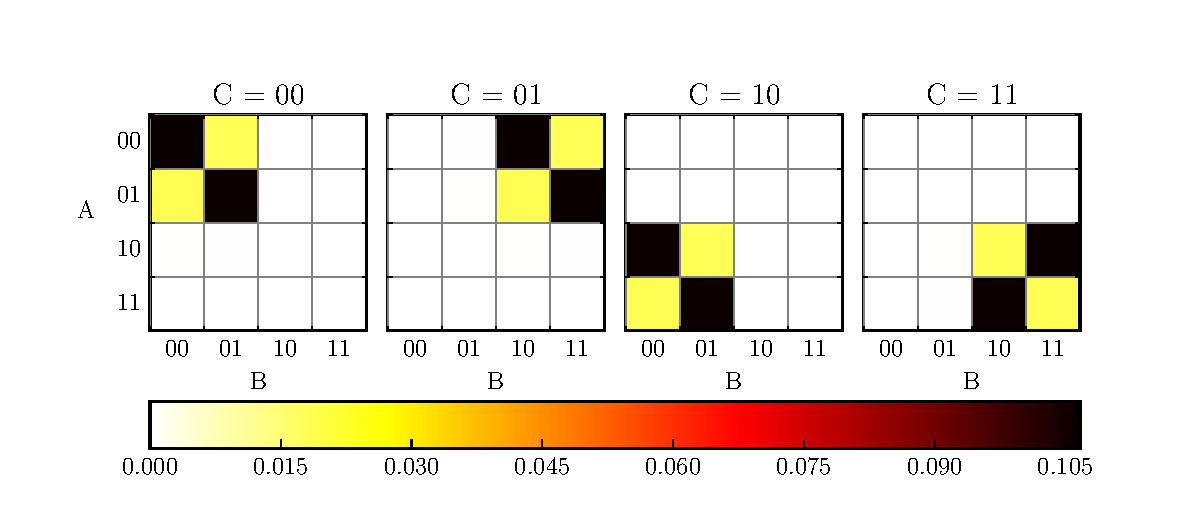
\includegraphics[scale=0.6]{../../figures/distributions/fritz_dist_plotted_bits.pdf}
            \vspace{-0.2in}
            \[ \probplotvalue{253, 253, 84} = \f{1}{32}\br{2 - \sqrt{2}} \qquad \probplotvalue{11, 1, 0} = \f{1}{32}\br{2 + \sqrt{2}}\]
            \caption{The Fritz distribution visualized using a $4 \times 4 \times 4$ grid. The $4$ outcomes of $A,B,C$ are written in binary as a doublet of bits to illustrate that certain bits act as measurement pseudo-settings.}
            \label{fig:fritz_distribution_visualized}
    \end{center}
    \end{figure}
    Consequently, it is possible to define the correlation $\ba{\p A_r \p B_r}$ between the right-hand bits of $\p A$ and $\p B$:
    \[ \ba{\p A_r \p B_r} = \prob[\p A_r \p B_r][00] + \prob[\p A_r \p B_r][11] - \prob[\p A_r \p B_r][01] - \prob[\p A_r \p B_r][10] \]
    Provided that $C$ is perfectly correlated with $A_l$ and $B_l$, any Bell inequality for the Bell structure defined over $\p{A}, \p{B}, S_{\p{A}}, S_{\p{B}}$ can be directly converted to an inequality for the Triangle structure by performing a simple relabeling: $\p{A}, \p{B}, S_{\p{A}}, S_{\p{B}} \mapsto \p{A}_r, \p{B}_r, \p A_l, \p B_l$. As an example, the famous CHSH inequality~\cite{CHSH_Original} (\cref{eq:CHSH_ineq_orig}) constrains the correlation between the right-bits of $A$ and $B$,
    \[ \ba{\p A_r \p B_r|\p C = 00} + \ba{\p A_r \p B_r|\p C = 01} + \ba{\p A_r \p B_r|\p C = 10} - \ba{\p A_r \p B_r|\p C = 11} \leq 2 \eq \label{eq:CHSH_intriangle} \]
    Every compatible distribution $\prob[ABC]$ for which $C$ is perfectly correlated $A_l,B_l$ must satisfy \cref{eq:CHSH_intriangle}. Substituting the \cref{eq:fritz_dist} into \cref{eq:CHSH_intriangle} yields the maximal violation~\cite{Cirelson_1980}: $3 \br{1/\sqrt{2}} - \br{-1/\sqrt{2}} = 2\sqrt{2} \not \leq 2$. Therefore, we conclude the Fritz distribution is incompatible with the Triangle structure. Before continuing it is worth noting that \cref{eq:fritz_dist} is non-unique. Nonetheless for concreteness, \cref{eq:fritz_dist} is taken as \textit{the} Fritz distribution throughout this manuscript.

    It is important to understand the domain in which Fritz's proof of incompatibility is valid; the details of which can found in the original work~\cite{Fritz_2012}. Specifically, \cref{eq:CHSH_intriangle} only acts as a valid causal compatibility inequality for the Triangle structure if there exists perfect correlation between $\p C$'s outcomes and the measurement pseudo-settings (left-bits) of $\p A$ and $\p B$. As a result, the incompatibility proof employed by Fritz is not applicable to any distribution that significantly deviates from the Fritz distribution presented above. For example, if one combines \cref{eq:fritz_dist} with more and more uniform noise, at what point does the resultant distribution transition from incompatibility to compatibility? This question is partially answered in \cref{sec:noise}.

    Upon reflection, the Fritz distribution can be considered \textit{manufactured}. The phenomenology associated with Bell non-locality or Bell incompatibility are well understood; examining these distributions embedded in the Triangle structure offers no additional perspective onto the types of entanglement resources made accessible by quantum mechanics. Therefore, it is desirable to find incompatible quantum distributions that are qualitatively different than those previously considered for the Bell structure. Pursuant to this, \citet{Fritz_2012} presented the following problem~\cite[Problem 2.17]{Fritz_2012}:%TODO figure out best way to link to this problem

    \term{Fritz's Problem}: Find an example of non-classical quantum correlations in the Triangle structure together with a proof of its non-classicality which does not hinge on Bell’s theorem.

    Understandably, Fritz's Problem is stated ambiguously as it is not yet entirely clear how to distinguish between non-classical distributions on differing causal structures. The remainder of this paper focuses on our advancement toward solving Fritz's Problem. \Cref{sec:conclusions} proposes three refinements of Fritz's Problem which are to be labeled \ref{r:1},\ref{r:2} and \ref{r:3} respectively. Specifically, \ref{r:1} embodies the degree in which the results of \cref{sec:found_inequalities} solve Fritz's problem while \ref{r:2} and \ref{r:3} characterize interpretations of Fritz's Problem that remain partially solved.

    \section{Triangle Structure Inequalities}
    \label{sec:found_inequalities}

    \Cref{sec:causal_compatibility} defined causal compatibility inequalities while \cref{sec:fritz_distribution} recalled and discussed the Fritz distribution together with a brief summary of its incompatibility with the Triangle Structure. Heretofore, there were no known causal compatibility inequalities for the Triangle Structure that were capable of witnessing the non-classicality of any quantum distributions~\cite{Inflation}. By leveraging the incompatibility of the Fritz distribution~\cite{Fritz_2012} and tools provided by the Inflation Technique~\cite{Inflation}, we have obtained numerous causal compatibility inequalities for the Triangle Structure that are violated by the Fritz distribution. A representative sample of these inequalities are presented here. The methods used to derive these inequalities are largely based on the Inflation Technique~\cite{Inflation}. A summary of the Inflation Technique and other methods used will be deferred to \cref{sec:inflation_technique} where unfamiliar readers will find a succinct yet sufficient presentation of the requisites.

    The first causal compatibility inequality is reported below:
    \begin{equation*}
    \begin{gathered}
    \eq\label{eq:ww_ineq}
    2P_{ABC}(203)P_{C}(0) + 2P_{ABC}(303)P_{C}(0) + P_{ABC}(003)P_{C}(0) + P_{ABC}(013)P_{C}(0) + \cdots \\
    \cdots + P_{ABC}(020)P_{C}(2) + P_{ABC}(022)P_{C}(2) + P_{ABC}(023)P_{C}(0) + P_{ABC}(023)P_{C}(2) + \cdots \\
    \cdots + P_{ABC}(030)P_{C}(2) + P_{ABC}(031)P_{C}(2) + P_{ABC}(032)P_{C}(2) + P_{ABC}(033)P_{C}(0) + \cdots \\
    \cdots + P_{ABC}(033)P_{C}(2) + P_{ABC}(103)P_{C}(0) + P_{ABC}(113)P_{C}(0) + P_{ABC}(123)P_{C}(0) + \cdots \\
    \cdots + P_{ABC}(133)P_{C}(0) + P_{ABC}(200)P_{C}(0) + P_{ABC}(200)P_{C}(1) + P_{ABC}(200)P_{C}(2) + \cdots \\
    \cdots + P_{ABC}(200)P_{C}(3) + P_{ABC}(201)P_{C}(0) + P_{ABC}(201)P_{C}(1) + P_{ABC}(201)P_{C}(2) + \cdots \\
    \cdots + P_{ABC}(201)P_{C}(3) + P_{ABC}(203)P_{C}(1) + P_{ABC}(203)P_{C}(2) + P_{ABC}(203)P_{C}(3) + \cdots \\
    \cdots + P_{ABC}(213)P_{C}(0) + P_{ABC}(223)P_{C}(0) + P_{ABC}(300)P_{C}(0) + P_{ABC}(300)P_{C}(1) + \cdots \\
    \cdots + P_{ABC}(300)P_{C}(2) + P_{ABC}(300)P_{C}(3) + P_{ABC}(301)P_{C}(0) + P_{ABC}(301)P_{C}(1) + \cdots \\
    \cdots + P_{ABC}(301)P_{C}(2) + P_{ABC}(301)P_{C}(3) + P_{ABC}(302)P_{C}(1) + P_{ABC}(303)P_{C}(1) + \cdots \\
    \cdots + P_{ABC}(303)P_{C}(2) + P_{ABC}(303)P_{C}(3) + P_{ABC}(313)P_{C}(0) - P_{ABC}(000)P_{C}(3) \geq 0
    \end{gathered}
    \end{equation*}
    By construction, every distribution $\prob[ABC]$ that is compatible with the Triangle Structure (i.e. factorizes according to \cref{eq:compatibility_as_factorization}) must satisfy \cref{eq:ww_ineq}. As a demonstration, the Fritz distribution violates \cref{eq:ww_ineq}. Notice the final term $\prob[ABC]\br{000}\prob[C]\br{3}$ has a coefficient $-1$. For the Fritz distribution, $\prob[ABC]\br{000}\prob[C]\br{3} = \f{1}{128}\br{2 + \sqrt{2}} \simeq 0.0267$ but all of the remaining terms in \cref{eq:ww_ineq} sum to $\simeq 0.0136$ meaning that the Fritz distribution violates this inequality with violation $-0.0129\ldots \not \geq 0$. Consequently we conclude that the Fritz distribution is incompatible with the Triangle Structure, a fact that was previously only demonstrated without the use of causal compatibility inequalities.

    To reiterate, the methods used to derive \cref{eq:ww_ineq} can be found in \cref{sec:marginal_satisfiability,sec:inflation_technique_main_summary} and more details can be found in \cref{sec:exemplary_inflations_of_the_triangle structure}.

    It is possible to simplify \cref{eq:ww_ineq} identifying sets of terms such as $P_{ABC}(300)P_{C}(0) + P_{ABC}(300)P_{C}(1) + P_{ABC}(300)P_{C}(2) + P_{ABC}(300)P_{C}(3)$ which can be simplified to $P_{ABC}(300)$ by recognizing that $P_{C}(0) + P_{C}(1) + P_{C}(2) + P_{C}(3) = 1$. Upon doing so, one obtains the following,
    \begin{gather*}
        P_{ABC}(303)P_{C}(0) + P_{ABC}(313)P_{C}(0) + P_{ABC}(302)P_{C}(1) + P_{AB}(02)P_{C}(2) + P_{AB}(03)P_{C}(2) + \cdots \\
        \cdots + P_{AB}(20) + P_{AB}(30) + P_{C}(3)P_{C}(0) - P_{ABC}(000)P_{C}(3) - P_{ABC}(021)P_{C}(2) + \cdots \\
        \cdots - P_{ABC}(202) - P_{ABC}(302) - P_{ABC}(233)P_{C}(0) - P_{AC}(33)P_{C}(0) \geq 0
    \end{gather*}

    In order to understand the importance of \cref{eq:ww_ineq}, there are a couple of important concepts to understand. First, the Fritz distribution was originally known to be incompatible with the Triangle structure due to the perfect correlation between $C$ and the measurement pseudo-settings $A_l, B_l$. The inequality of \cref{eq:ww_ineq} represents a significant advancement in our understanding of non-classicality in the Triangle structure. For example, \cref{eq:ww_ineq} is violated by distributions that do not exhibit perfect correlation between $C$ and $A_l, B_l$. Furthermore, the existence of an inequality capable of witnessing Fritz distribution \textit{is guaranteed}, albeit there was \textit{no guarantee} that the Inflation Technique would be capable of producing such an inequality. In fact, \cref{eq:ww_ineq} was derived using the Wagon-Wheel inflation depicted in \cref{fig:wagon_wheel_inflation}; smaller inflations of the Triangle structure such as the Spiral inflation (\cref{fig:spiral_inflation}) and Cut inflation (\cref{fig:cut_inflation}) are \textit{not} able to produce causal compatibility inequalities that witness the Fritz distribution. This result demonstrates that the Inflation Technique is the first tool-set powerful enough to produce causal compatibility inequalities such as \cref{eq:ww_ineq} strong enough to witness incompatible quantum distributions for the Triangle Structure. More universally, this result shows that the Inflation Technique is a promising tool for understanding quantum non-classical in more general causal structures.

    In addition to \cref{eq:ww_ineq}, numerous independent inequalities were derived for the Triangle Structure that are violated by the Fritz distribution. The majority of these inequalities share most or all of the qualitative features of \cref{eq:ww_ineq}, and hence those inequalities are omitted from this manuscript. Instead, we present \cref{eq:web_inequality}, another causal compatibility inequality for the Triangle structure that is violated by the Fritz distribution and was produced using the \cref{fig:the_web_inflation} --- a considerably larger inflation than the Wagon-Wheel inflation. Note that in \cref{eq:web_inequality} $\prob\br{abc}$ is shorthand for $\prob[ABC]\br{abc}$.

    \begin{equation}
        \label{eq:web_inequality}
        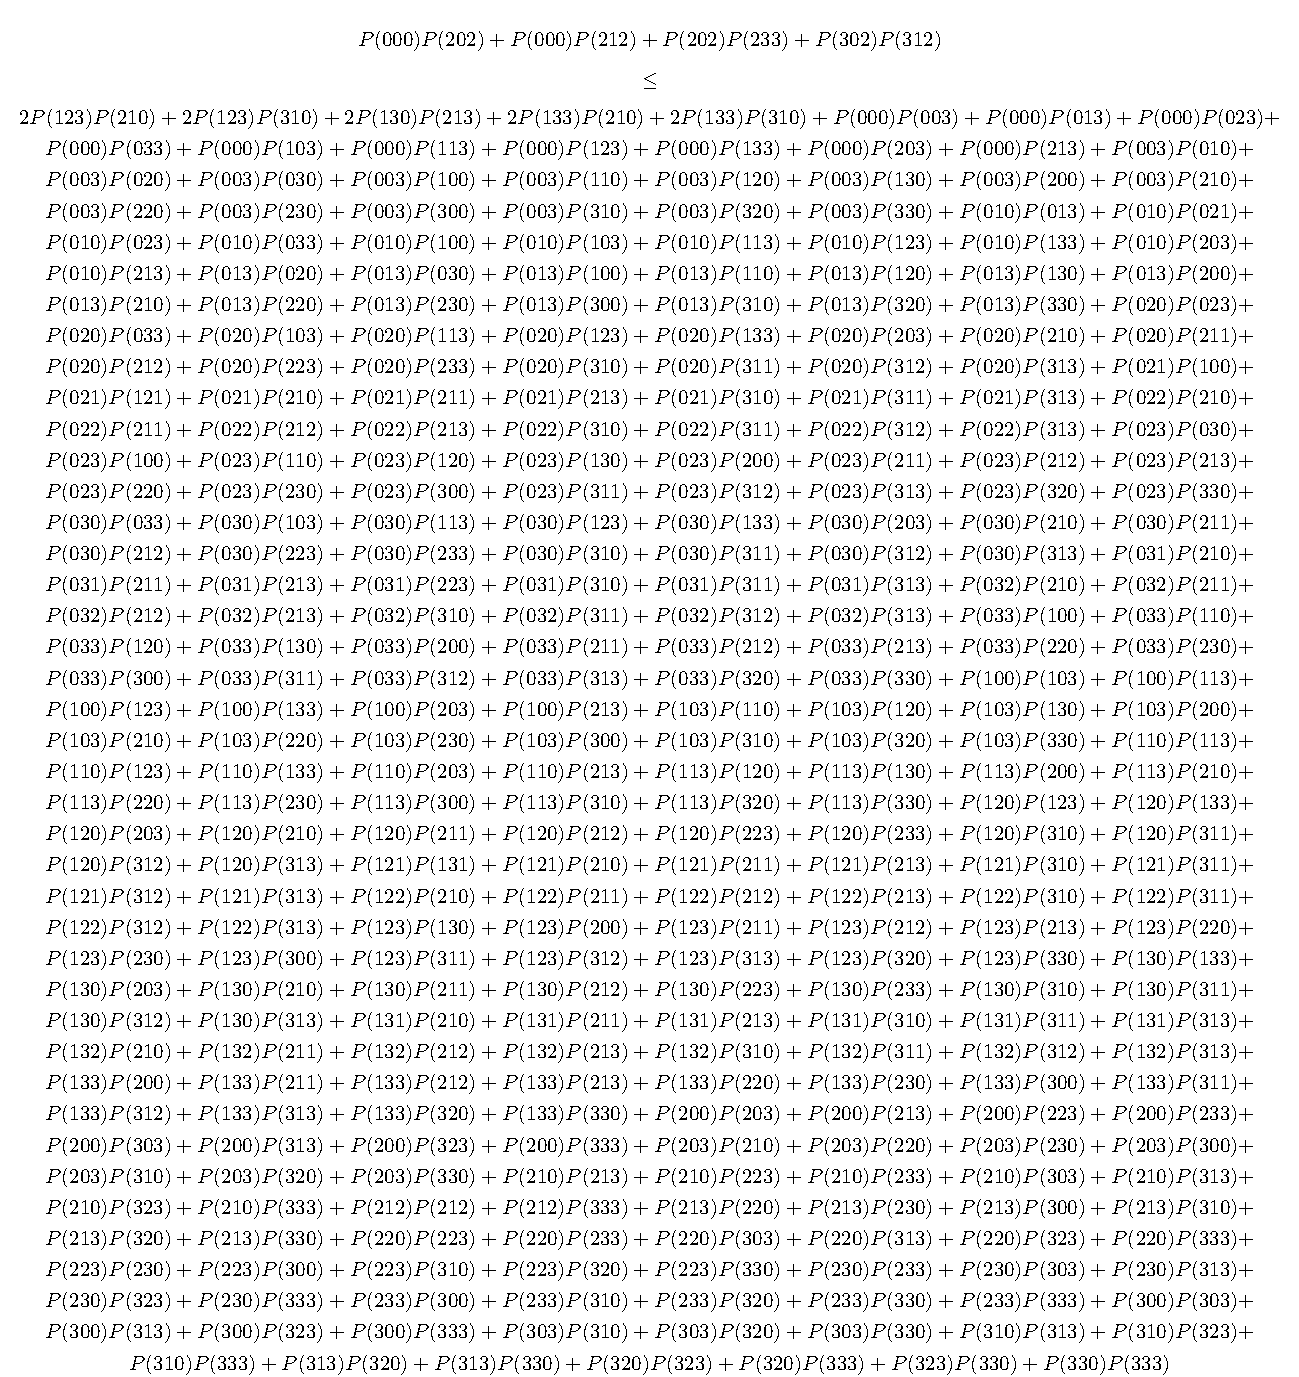
\includegraphics[width=\linewidth]{../../figures/inequalities/no_symwitness_ineq_print_standalone}
    \end{equation}

    The inequalities presented above (\cref{eq:ww_ineq,eq:web_inequality}) were curated to demonstrate the incompatibility of the Fritz distribution in particular. To reiterate, the Fritz distribution is incompatible with the Triangle Structure because it assigns a unique role to one of the variables, specifically $C$. The asymmetry within the Fritz distribution is reflected in the asymmetry of \cref{eq:ww_ineq,eq:web_inequality}. In order to discover new forms of non-classicality in the Triangle Structure, it is desirable to obtain measures of non-classicality (i.e. inequalities) that do not admit this bias. In an effort to find a causal compatibility inequality qualitatively distinct from \cref{eq:ww_ineq,eq:web_inequality}, we developed a technique to derive inequalities with certain symmetry properties such as \cref{eq:symmetic_web_inequality} which is symmetric with respect to any permutation of the variables $A, B, C$. These techniques are explained in \cref{sec:symmetric_inequalities}. Surprisingly, \cref{eq:symmetic_web_inequality} is also violated by the Fritz distribution.
    \begin{equation}
        \label{eq:symmetic_web_inequality}
        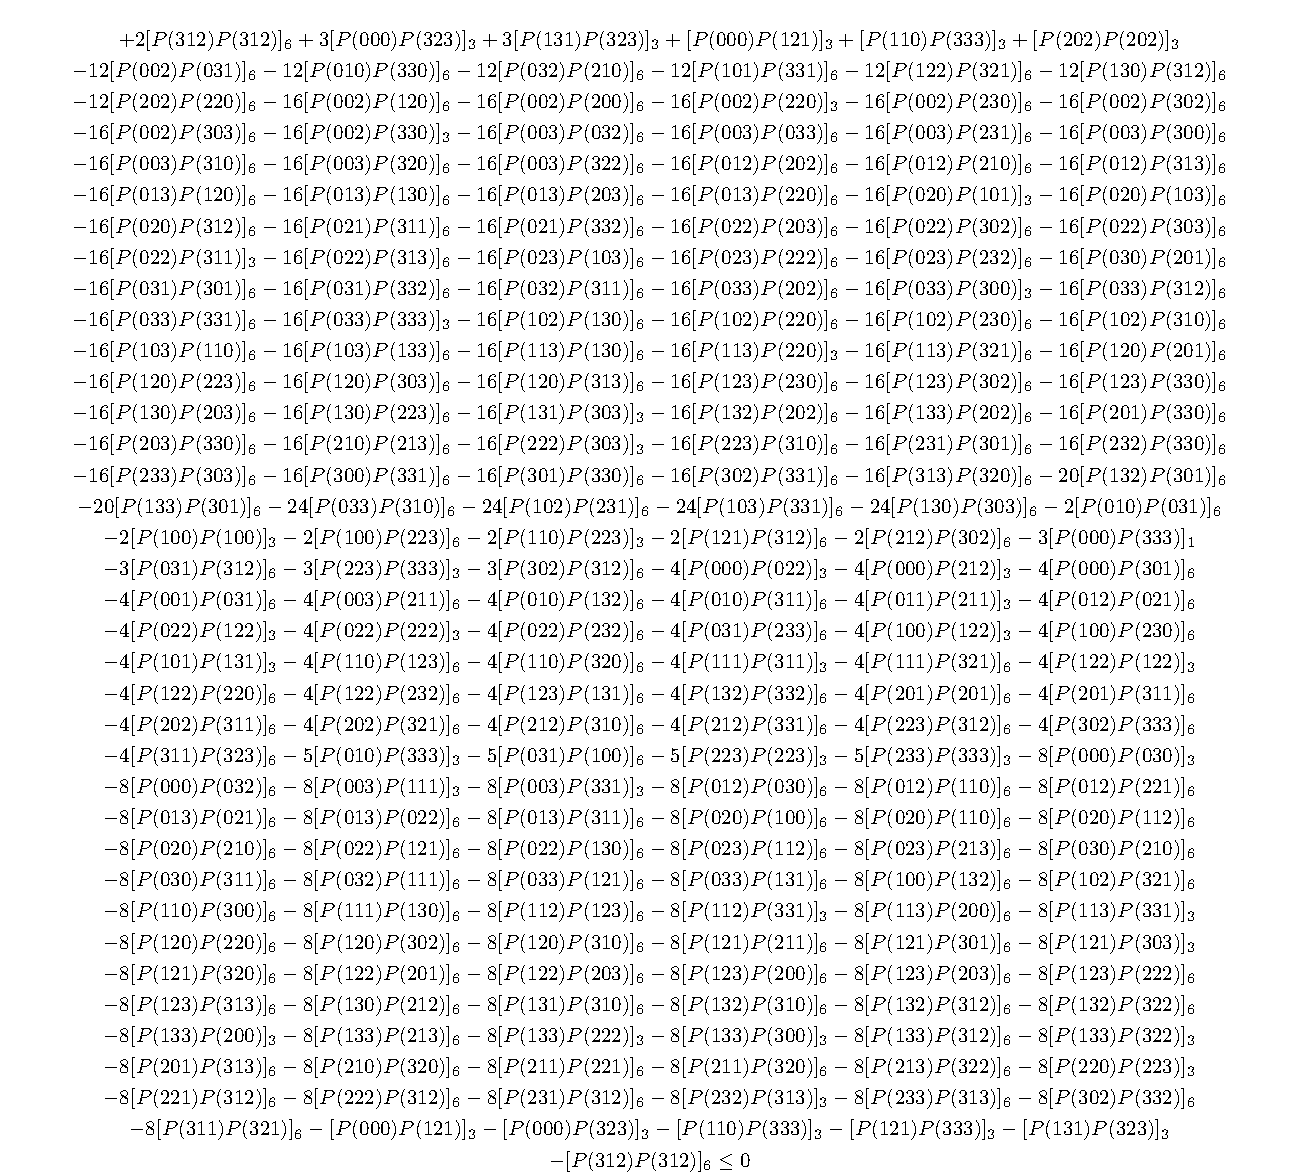
\includegraphics[width=\linewidth]{../../figures/inequalities/MosekCertFritzSym_ineq_standalone}
    \end{equation}
    Note that $\prob\br{abc}$ is shorthand for $\prob[ABC]\br{abc}$ and $\bs{P(113)P(330)}_3$ is shorthand for a sum the over permutations of $A,B,C$, i.e. $\bs{P(113)P(330)}_3 \defined P(113)P(330) + P(131)P(303) + P(311)P(033)$.

    Most importantly, these causal compatibility inequalities are a positive resolution of Fritz's problem from \cref{sec:fritz_distribution}. These inequalities are derived without making use of Bell's theorem and instead uses the Inflation Technique to approach non-classicality from a causal inference perspective. Additionally, the derivation of causal compatibility inequalities allows one prove incompatibility even when perfect correlations are absent.

    \section{Numerical Optimizations \& Noisy Distributions}
    \label{sec:violations_noise}
    Causal compatibility inequalities for the Triangle structure (such as those derived in \cref{sec:deriving_inequalities}) offer an avenue into studying quantum non-classicality. In this section, we make use of two methods, exposure to noise and numerical optimization, to further understand the nature of quantum non-classicality in connection to compatibility inequalities. In order to compare different inequalities simultaneously, our convention is to rearrange each inequality $I$ so $I\br{\prob} < 0$ represent a violation of $I$ while $I\br{\prob} \leq 0$ represents satisfaction of $I$ (with $I\br{\prob} = 0$ corresponding to complete saturation of the inequality). For the subsequent analysis, $4$ inequalities where chosen. First, $I_0$ is the inequality derived using the Wagon-Wheel wheel inflation \cref{eq:ww_ineq}. The other three inequalities $I_1, I_2, I_3$ were all derived using the Web inflation; $I_1$ can be found in \cref{eq:web_inequality} while $I_3$ is the symmetric inequality in \cref{eq:symmetic_web_inequality}. Inequality $I_2$ is not reproduced anywhere in this document but is similar to \cref{eq:web_inequality}.

    \subsection{Noisy Distributions}
    \label{sec:noise}
    % \begin{figure}
    % \begin{center}
    %         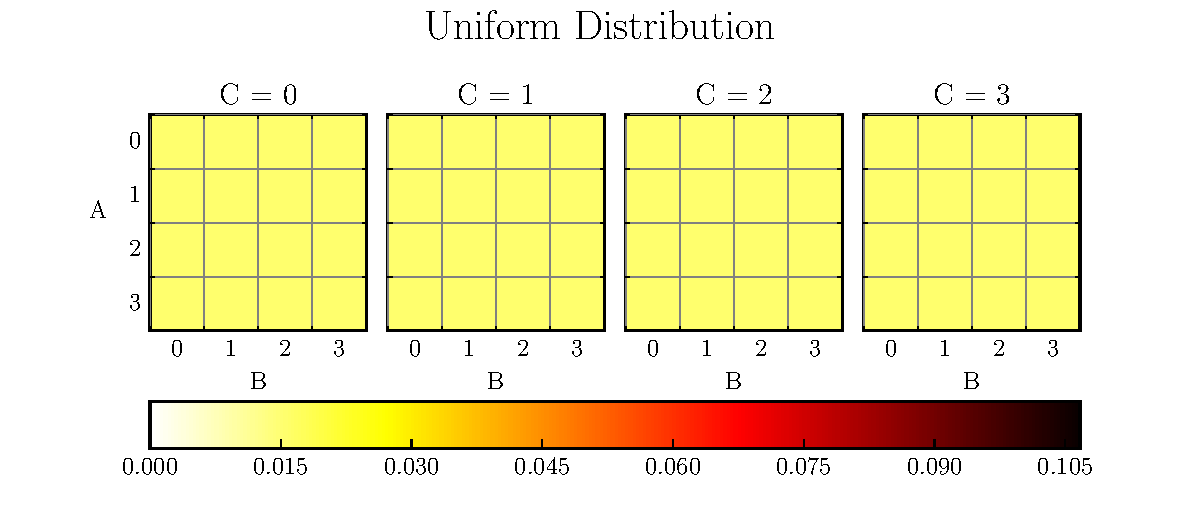
\includegraphics[scale=0.6,trim={0 0 0 0.4in},clip]{../../figures/distributions/uniform_dist_plot.pdf}
    %         \vspace{-0.2in}
    %         \[ \probplotvalue{255, 255, 109} = \f{1}{64} \]
    %         \caption{The completely uniform distribution $\s{U}$ visualized using a $4 \times 4 \times 4$ grid.}
    %         \label{fig:uniform_distribution}
    % \end{center}
    % \end{figure}
    In his original work, \citet{Fritz_2012} was able to find quantum non-classicality in the Triangle structure by embedding Bell non-classicality. As was mentioned in \cref{sec:fritz_distribution}, this embedding required a very idealistic condition to hold: perfect correlations between $C$ and $A_l, B_l$. From an experimental point of view, it is impossible to use Fritz's original argument to confirm non-classicality because every observable distribution is subject to \text{noise}. It is possible to minimize noise by developing more accurate measurement channels but perfect correlations are too idealistic. Causal compatibility inequalities not only permit there to be noise within a set of observations, but they also provide a means of quantifying the amount of noise that is allowed before non-classicality breaks down.

    For Triangle structure, we define a completely noisy observation as the uniform probability distribution $\s{U}\br{abc} = \s{U}_{ABC}\br{abc} = \f{1}{64} \quad \forall a,b,c\in \bc{0,1,2,3}$. Since the uniform distribution $\s{U}$ is trivially compatible with the Triangle structure, the objective of this section is to determine how much uniform noise needs to be added to the Fritz distribution $\prob[\fritz]$ before it transitions from incompatible to compatible. We do this by defining an affine noise parameter $\vep$ such that $0 \leq \vep \leq 1$ along with the \term{noisy variant} $\s{N}_{\vep}$ of the Fritz distribution,
    \[ \s{N}_{\vep} = \br{1 - \vep} \prob[\fritz] + \vep \s{U} \]
    Therefore as $\vep$ varies from $0$ to $1$, more and more noise is added to the Fritz distribution and $\s{N}_{\vep}$ transitions from an incompatible distribution $\s{N}_{0} = \prob[\fritz]$ to a compatible distribution $\s{N}_{1} = \s{U}$. For each inequality $I$ and distribution $\prob$, let $I\br{\prob}$ denote a scalar value representing the amount of violation seen by $\prob$.  Our tests suggest that inequality $I_1$ (\cref{eq:web_inequality}) is most robust to noise and demonstrates that the Fritz distribution remains incompatible with the Triangle structure up to at least a noise parameter of $\vep \simeq 0.085$. The associated distribution $\s N_{0.085}$ is plotted in \cref{fig:noisy_fritz}. Of course, there remains the possibility that another inequality will be able to withstand a larger degree of noise than $I_1$.

    % Given that $I_0, I_1, I_2, I_3$ are far from a representative inequalities and are likely not facets of any inflated marginal polytope, it is save to say that this is possible.

    % \begin{figure}
    % \begin{subfigure}[b]{.48\linewidth}
    % {\centering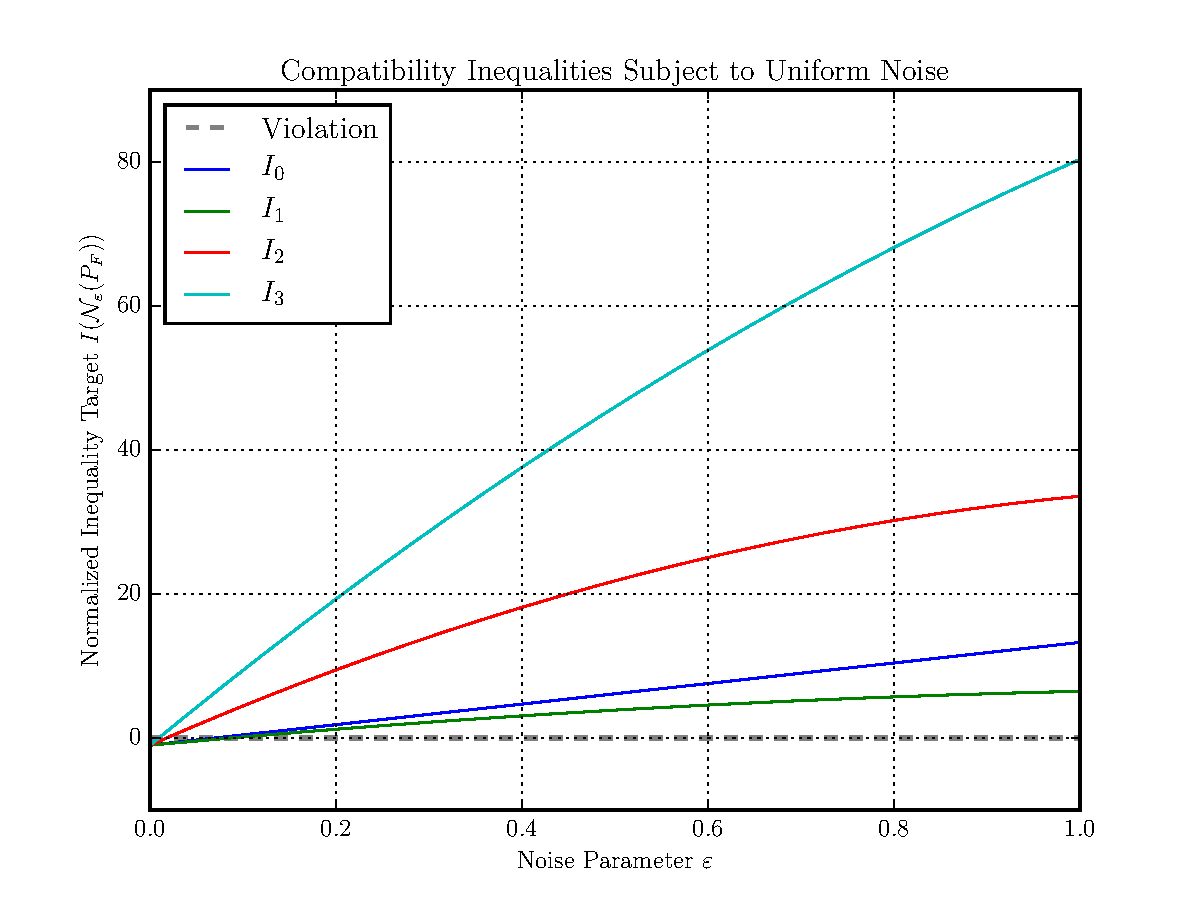
\includegraphics[width=\linewidth]{../../figures/noise/noise_2017.pdf}}
    % \caption{Complete range of noise parameters $\vep$.}\label{fig:noise}
    % \end{subfigure}
    % \begin{subfigure}[b]{.48\linewidth}
    % {\centering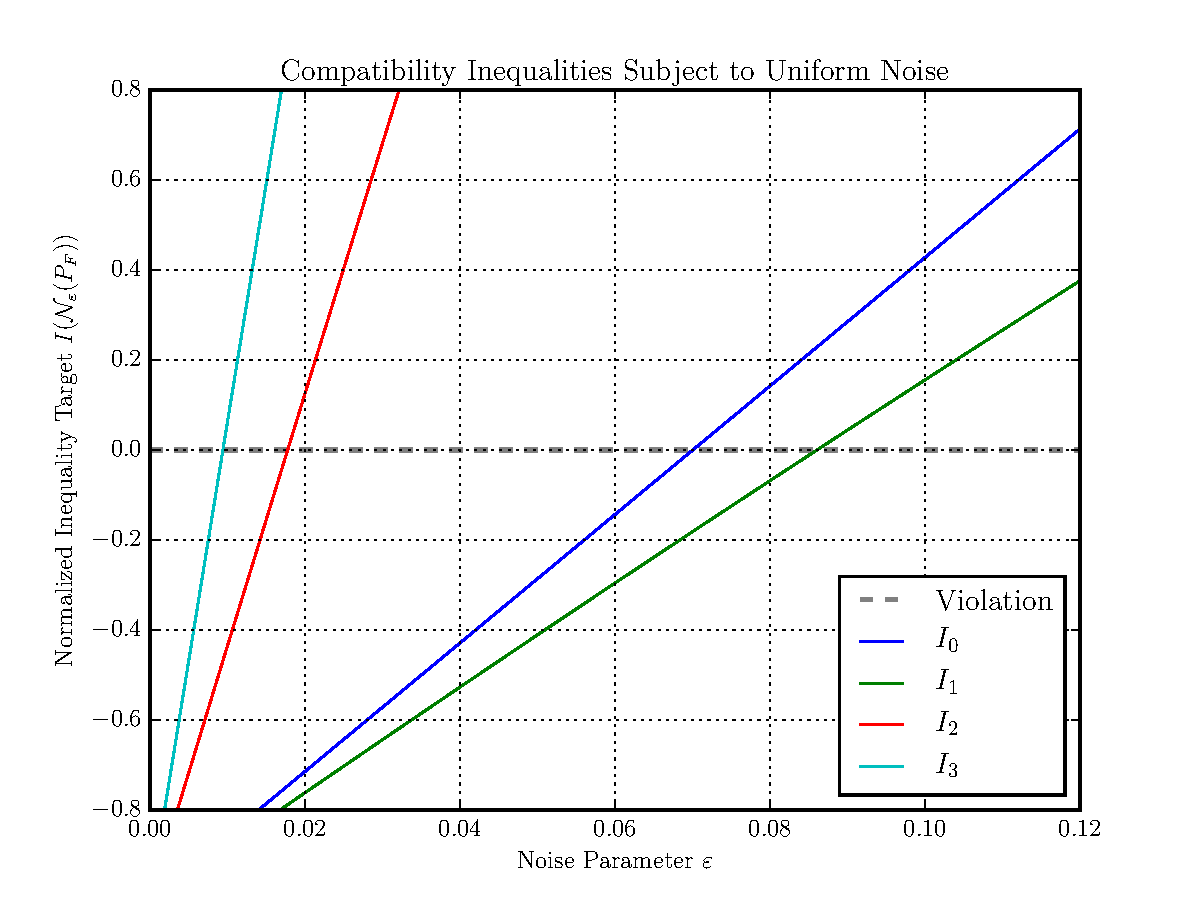
\includegraphics[width=\linewidth]{../../figures/noise/noise_2017_lims.pdf}}
    % \caption{\Cref{fig:noise} zoomed onto relevant region.}\label{fig:noise_zoomed}
    % \end{subfigure}
    % \caption{Inequality violations when subjected to uniform noise. Each inequality is normalized so that maximum violation is $-1$.}\label{fig:master_noise}
    % \end{figure}

    % The results of our experiments are plotted in \cref{fig:master_noise}. \Cref{fig:noise} illustrates that each curve $I\br{\s{N}_{\vep}\br{\prob[\fritz]}}$ as a function of $\vep$ is monotonically increasing as expected; the more noise added to the probability distribution, the more classical it becomes. \Cref{fig:noise_zoomed} is the same plot as \cref{fig:noise} zoomed onto the interval $\vep \in \bs{0, 0.12}$.



    \begin{figure}
    \begin{center}
            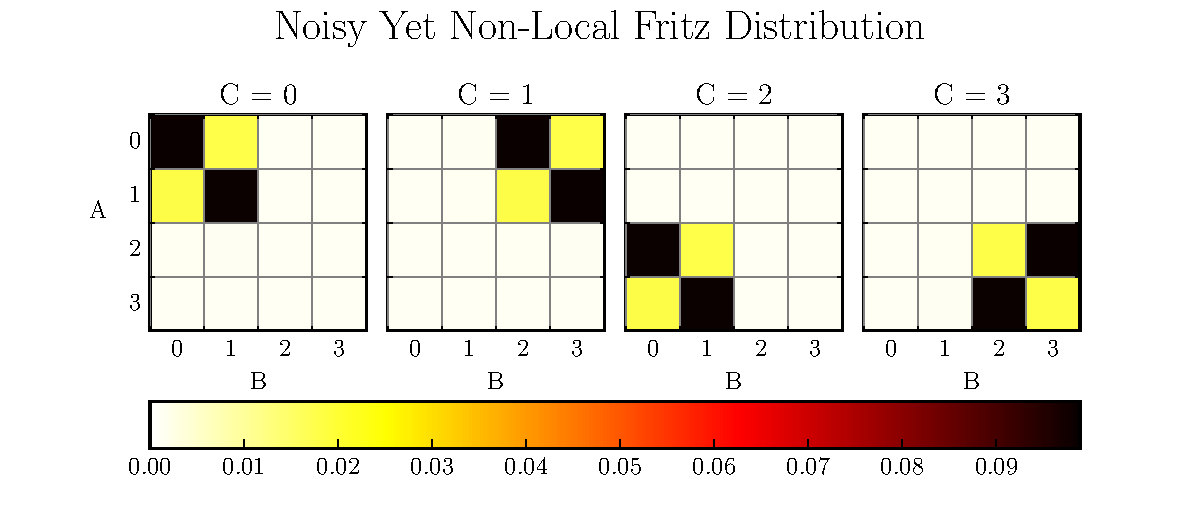
\includegraphics[scale=0.6,trim={0 0 0 0.4in},clip]{../../figures/noise/noisy_yet_non_local_fritz.pdf}
            \vspace{-0.2in}
            \[ \probplotvalue{255, 255, 243} = 0.00133 \]
            \caption{$\s{N}_{0.085}$: A noisy yet still non-classical variant of the Fritz distribution.}
            \label{fig:noisy_fritz}
    \end{center}
    \end{figure}

    \subsection{Numerical Optimizations}
    \label{sec:optimizations}
    \todo[TC]{Determine if I should remove this paragraph or shorten it}
    Causal compatibility inequalities act as a \textit{measure} of non-classicality. If two non-classical distributions $\prob[1]$ and $\prob[2]$ violate the same inequality $I$ with violations $I\br{\prob[1]}$ and $I\br{\prob[2]}$ respectively, it is somewhat reasonable to say that $\prob[1]$ is \textit{more} non-classical than $\prob[2]$ whenever ${I\br{\prob[1]}} < I\br{\prob[2]}$. However, this statement is accompanied by a few caveats. First, it is possible (and frequently the case) for ${I\br{\prob[1]}} < I\br{\prob[2]}$ to hold for one inequality $I$ but have ${\ti I\br{\prob[2]}} < \ti I\br{\prob[1]}$ hold for another inequality $\ti I$. In this case, all one can claim is that $\prob[1]$ is more incompatible than $\prob[2]$ with respective to $I$ but the contrary is true with respect to $\ti I$. Second, not all inequalities $I$ are \textit{good} measures of non-classicality. In the case of the Bell structure, the linear inequality constraints associated with the facets of the marginal polytope are the best measures of non-classicality because the facets form a necessary and sufficient of constraints with all other inequalities following from positive mixtures. However, good measures of incompatibility are less understood in the Triangle structure where the space of classical correlations is non-convex. At the very least, the inequalities derived in this report are likely \textit{not} the best measures of incompatibility simply because they have be curated toward the Fritz distribution. Nonetheless, these inequalities act the \textit{first} measures of non-classicality in the Triangle structure.

    In order to find quantum distributions that are more non-classical than the Fritz, we performed numerical optimizations against each inequality $I$ by parameterizing the space of quantum-accessible probability distributions that can be realized on the Triangle Structure \cref{fig:triangle_structure} and thus expressed as follows:
    \[ \prob[\p{ABC}]\br{abc} = \Tr\bs{\netperm^\intercal \rho_{\p{AB}}\otimes\rho_{\p{BC}}\otimes\rho_{\p{CA}} \netperm M_{\p{A},a}\otimes M_{\p{B},b} \otimes M_{\p{C},c}} \eq \label{eq:quantum_model_triangle}\]
    Where $\rho_{\p{AB}}, \rho_{\p{BC}}, \rho_{\p{CA}}$ are bipartite density matrices, $M_{\p{A}}, M_{\p{B}}, M_{\p{C}}$ are generic measurements sets and $\netperm$ is a permutation matrix that aligns the states and measurements appropriately. In order to parameterize all such distributions, we elect to parameterize the states and measurements separately. In order to qualify the scope of \cref{eq:quantum_model_triangle} and associated computational complexity of the parameterization, there are a two restrictions that are made with justification. Motivated by the fact that the Fritz distribution (\cref{sec:fritz_distribution}) only requires qubit states, the states $\rho$ are taken to be bipartite \textit{qubit} states. Qubit states are more computationally feasible compared to $n$-dimensional states whereby the joint density matrix $\rho_{\p{AB}}\otimes\rho_{\p{BC}}\otimes\rho_{\p{CA}}$ becomes an $n^6 \times n^6$ matrix. Additionally, we restrict our focus to projective-valued measures (PVMs) instead of projective-operator valued measures (POVMs) for three reasons. First, \cref{sec:fritz_distribution} demonstrates that PVMs are sufficient for witnessing incompatible quantum distributions in the Triangle structure. Second, although generating $k$-outcome POVM measurements is possible using rejection sampling techniques~\cite{Petz_2015}, a valid, unbiased parameterization was not found for $k > 2$. Finally, PVMs provide considerable computational advantage over POVMs as they permit \cref{eq:quantum_model_triangle} to be re-written as \cref{eq:quantum_model_triangle_pvms}.
    \[ \prob[\p{ABC}]\br{abc} = \bramidket{m_{\p{A},a}m_{\p{B},b}m_{\p{C},c}}{\netperm^\intercal \rho_{AB}\otimes\rho_{BC}\otimes\rho_{CA} \netperm}{m_{\p{A},a}m_{\p{B},b}m_{\p{C},c}} \eq \label{eq:quantum_model_triangle_pvms}\]

    Although there are numerous techniques that can used when parameterizing quantum states and measurements~\cite{Petz_2015, Hedemann_2013,Fujii_2005,James_2001,Grasmair_2014,Neilsen_Chaung_2011}, a single technique by \citet{Spengler_2010_Unitary} was found to be most computationally suitable for our purposes. \Citet{Spengler_2010_Unitary} demonstrated that all $d\times d$ unitary matrices $U$ can be parameterized without degeneracy as follows:
    \[ U = \bs{\prod_{m=1}^{d-1} \br{\prod_{n=m+1}^{d} \exp\br{i P_n \lambda_{n,m}}\exp\br{i \si_{m,n} \lambda_{m,n}}}} \cdot \bs{\prod_{l=1}^{d} \exp\br{iP_l \lambda_{l,l}}}  \eq \label{eq:spengler_unitary} \]
    Where the real valued parameters $\la = \bc{\la_{n,m} \mid n,m \in 1, \ldots, d}$ have periodicities $\la_{m,n} \in \bs{0, \f{\pi}{2}}$ for $m < n$ and $\la_{m,n} \in \bs{0, 2 \pi}$ for $m \geq n$. Moreover, $P_l$ are one-dimensional projective operators $P_l = \ket{l}\bra{l}$ and the $\si_{m,n}$ are generalized anti-symmetric $\si$-matrices $\sigma_{m,n} = -i \ket{m}\bra{n} +i \ket{n}\bra{m}$ where $1 \leq m < n \leq d$. This parameterization has the useful feature that each of the real-valued parameters $\la_{n,m}$ a direct and intuitive physical affect on each element of a computational basis $\bc{\ket{1}, \ldots, \ket{d}}$. Explicitly, $\exp\br{i \si_{m,n} \lambda_{m,n}}$ applies a rotation to the sub-space spanned by $\ket{m}$ and $\ket{n}$ for $m < n$. Analogously, $\exp\br{i P_n \lambda_{n,m}}$ generates the relative phase between $\ket{m}$ and $\ket{n}$ for $m > n$ and $\exp\br{iP_l \lambda_{l,l}}$ fixes the global phase of $\ket{l}$. Finally, although not explicitly mentioned in~\cite{Spengler_2010_Unitary}, it is possible to remove the reliance on the computationally expensive matrix exponential operations in \cref{eq:spengler_unitary}~\cite{Moler_2003}.

    By parameterizing unitary matrices, it becomes possible to parameterize $d$-dimensional density matrices and $d$-element PVMs by recognizing that any orthonormal basis $\bc{\ket{\psi_j}}$ (where $1 \leq j \leq d$) can be transformed into the computational basis $\bc{\ket{j}}$ by a unitary transformation $U$, i.e. $U \ket{\psi_j} = \ket{j}$. First consider a $d$-element PVM $M = \bc{\ket{m_j}\bra{m_j} \mid 1 \leq j \leq d}$. Since $\bc{\ket{m_j}}$ forms an orthonormal basis, one can parameterize $M$ by writing $M = \bc{U^{\dagger}\ket{j}\bra{j}U \mid 1 \leq j \leq d}$ and parameterizing $U$ using \cref{eq:spengler_unitary}. This method was inspired by the measurement seeding method for iterative optimization used by \citet{Pal_2010}. Analogously, this argument can be extended to full-rank $d$-dimensional density matrices $\rho$ by performing a spectral decomposition $\rho = \sum_{j=1}^{d} p_j \ket{p_j} \bra{p_j}$ into eigenvalues $\bc{p_j}$ and eigenstates $\bc{\ket{p_j}}$. Since $\Tr\br{\rho} = \sum_{j = 1}^{d} p_j = 1$ the eigenvalues of $\rho$ are parameterized without degeneracy using a tuple of $d-1$ real-valued parameters with periodicity $\bs{0, 2 \pi}$ using hyper-spherical coordinates~\cite{Hedemann_2013, Spengler_2010_Unitary}. Additionally, since $\rho$ is Hermitian, the eigenstates $\bc{\ket{p_j}}$ form an orthonormal basis and therefore the eigenstates are analogously parameterized using \cref{eq:spengler_unitary}: $\rho = \sum_{j=1}^{d} p_j U^{\dagger} \ket{j} \bra{j} U$. For our purposes, we have set $d = 4$ and fixed $\la_{l, l} = 0$ for $1 \leq l \leq d$ in \cref{eq:spengler_unitary} because the global phase contributions are irrelevant for \cref{eq:quantum_model_triangle_pvms}.

    % \Cref{sec:param_quantum_dist} expounds on our parameterized of the space of quantum distributions that can be realized on the quantum Triangle structure (\cref{fig:triangle_structure_quantum_model}) pursuant to \cref{eq:quantum_model_triangle_pvms}. Specifically, each bipartite quantum resource is modeled $2$-qubit, $4\times 4$ density matrix and each measurement is modeled as a $4$-element projective-value measure.

    % the a objective scalar function $f: \R^n \in \R$ using the following pipeline: To begin, a set of real-valued parameters $\la = \br{\la_0, \ldots, \la_n} \in \R^{n}$ are used to parameterize a set of quantum states $\rho_{AB}, \rho_{BC}, \rho_{CA}$ and measurements $M_A, M_B, M_C$ in agreement with the quantum version of the Triangle structure in \cref{fig:triangle_structure_quantum_model}. Second, a $4$-outcome distribution $\prob[ABC]$ is obtained via \cref{eq:quantum_model_triangle} and supplanted into an inequality $I$ in homogeneous and canonical form $I\br{\prob[ABC]} \leq 0$. The objective value is simply the degree of violation $f = I\br{\prob[ABC]}$ and used to make adjustments to $\la$ in order to achieve largest and larger violations.

    % \subsection{Parameterizing Quantum Distributions}
    % \begin{figure}
    % \begin{center}
    %         \scalebox{1.0}{\begin{tikzpicture}[scale=1]
    \begin{scope}[every node/.style=observed]
        \node (C) at (-2, 0) {$M_{\p{C}}$};
        \node (B) at (2, 0) {$M_{\p{B}}$};
        \node (A) at (0, {2*sqrt(3)}) {$M_{\p{A}}$};
    \end{scope}
    \begin{scope}[every node/.style=latent]
        \node (X) at (-1, {sqrt(3)}) {$\rho_{\p{CA}}$};
        \node (Y) at (1, {sqrt(3)}) {$\rho_{\p{AB}}$};
        \node (Z) at (0, 0) {$\rho_{\p{BC}}$};
    \end{scope}
    \begin{scope}[every path/.style={draw=cause, thick}]
        \path[postaction={on each segment={mid arrow}}]
        (X) -- (A)
        (X) -- (C)
        (Y) -- (A)
        (Y) -- (B)
        (Z) -- (B)
        (Z) -- (C);
    \end{scope}
\end{tikzpicture}}
    %         \caption{The Triangle structure as modeled by quantum states and measurements.}
    %         \label{fig:triangle_structure_quantum_model}
    % \end{center}
    % \end{figure}


    % \subsection{Numerical Optimization Results}

    \begin{figure}
    \begin{center}
            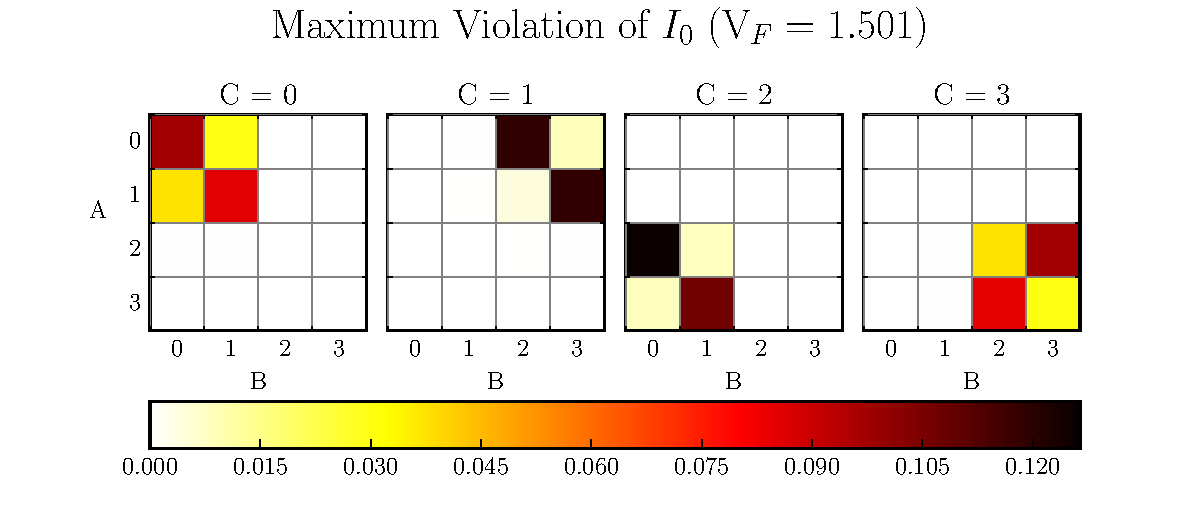
\includegraphics[scale=0.6,trim={0 0 0 0.4in},clip]{../../figures/distributions/plotted_dist_I_1_max_violation_2017.pdf}
            \caption{Probability distribution that maximizes violation of $I_1$ from \cref{eq:web_inequality} ($V_F \simeq 1.501$).}
            \label{fig:maximum_violation_I_1}
    \end{center}
    \end{figure}
    \begin{figure}
    \begin{center}
            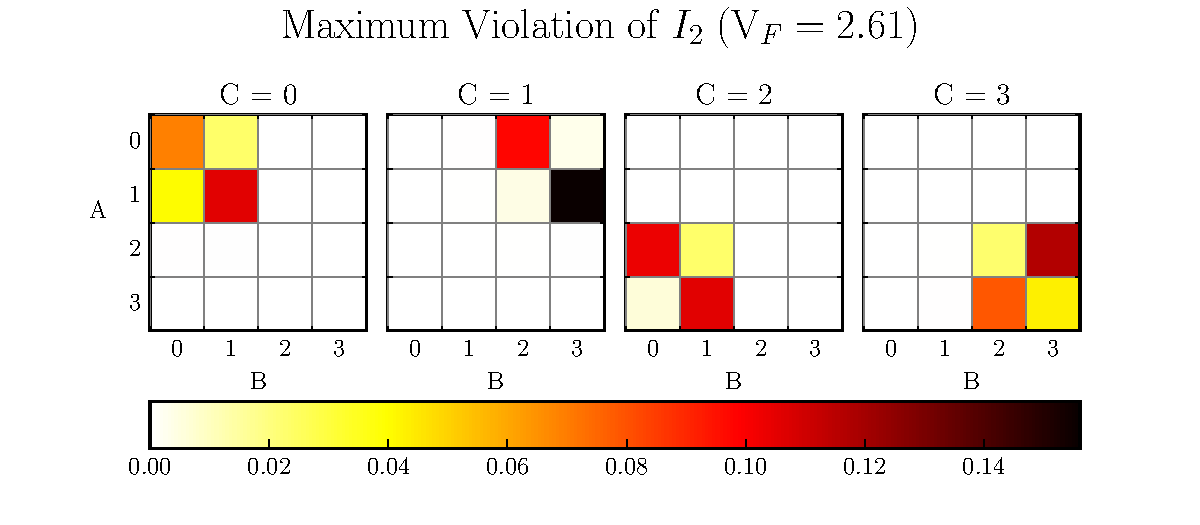
\includegraphics[scale=0.6,trim={0 0 0 0.4in},clip]{../../figures/distributions/plotted_dist_I_3_max_violation_2017.pdf}
            \caption{Probability distribution that maximizes violation of $I_3$ from \cref{eq:symmetic_web_inequality} ($V_F \simeq 2.61$).}
            \label{fig:maximum_violation_I_3}
    \end{center}
    \end{figure}
    \begin{figure}
    \begin{center}
            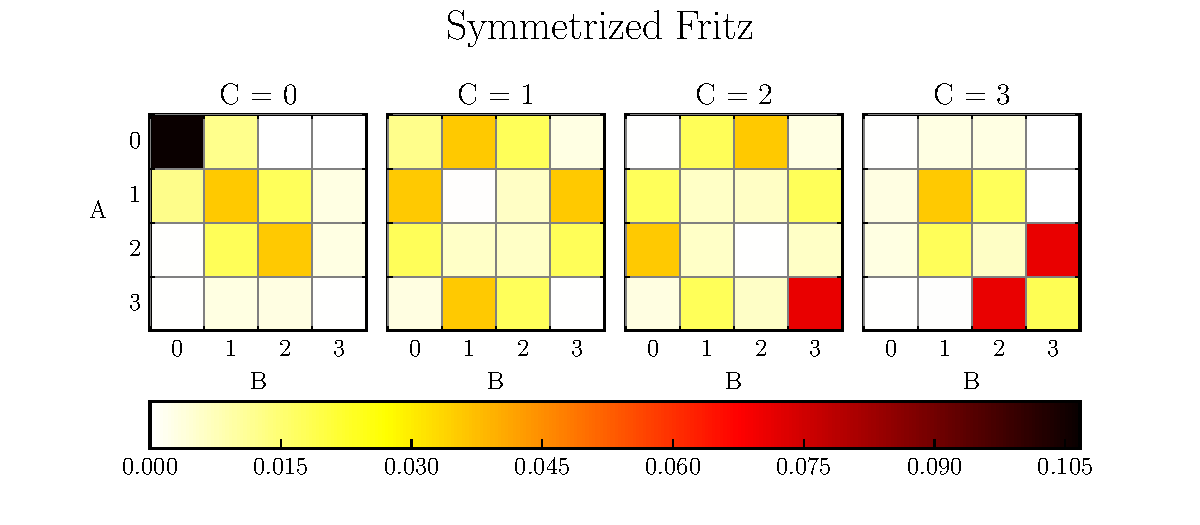
\includegraphics[scale=0.6,trim={0 0 0 0.4in},clip]{../../figures/distributions/symmetrized_fritz.pdf}
            \caption{Symmetrized version of the Fritz distribution ($V_F \simeq 3$).}
            \label{fig:symmetrized_fritz}
    \end{center}
    \end{figure}

    To quantify the degree in which each inequality $I$ could be further violated, we define a relative violation $V_F$ to be the maximum violation relative to the violation achieved by the Fritz distribution, i.e. $V_F \defined \min_{P}\bc{I\br{P}}/I\br{P_F}$. The first inequality in consideration is $I_1$; the non-symmetric Web inflation inequality presented in \cref{eq:web_inequality}. At best, numerical optimizations converged to a distribution (\cref{fig:maximum_violation_I_1}) with relative violation $V_F \simeq 1.501$. Almost immediately, it is evident that \cref{fig:maximum_violation_I_1} closely resembles the Fritz distribution. In fact, \cref{fig:maximum_violation_I_1} and \cref{fig:fritz_distribution_visualized} share the exact same \textit{possibilistic structure}, i.e. the same set of possible events. This result is not entirely unexpected. As was mentioned in \cref{sec:found_inequalities}, these inequalities are derived specifically to prove the incompatibility of the Fritz distribution and the Triangle structure. Consequently, it seems that $I_1$ only has the capacity to demonstrate incompatibility for distributions that resemble the Fritz distribution very closely.

    An alternative explanation for qualitative similarities between \cref{fig:maximum_violation_I_1} and \cref{fig:fritz_distribution_visualized} is related to the sensitively of the initial parameters to our optimization. Above it was shown that our parameter space of choice was $2\pi$-periodic in all entries. Somewhat surprisingly, when supplied with randomly sampled initial parameters, all optimization methods consistently converged to inequality \textit{saturation} instead of inequality \textit{violation} which is achievable by the Fritz distribution $\prob[\fritz]$. Instead, it was observed that only parameters close enough to the \textit{Fritz parameters} (i.e. any non-unique set of parameters that induce the Fritz distribution) were able to achieve violation. Since the inequalities themselves are polynomial and the space of quantum-accessible distributions is non-convex, a number of optimization methods were used in an attempt to eliminate any issues associated with local minima or ill-conditioned convergence. Specifically, the BFGS method~\cite[p.142]{Nocedal_2000} and the Nelder-Mead simplex method~\cite[p.238]{Nocedal_2000} were used along with a method called Basin Hopping~\cite{Wales_1997}, which is a hybrid between simulated annealing and gradient descent-based methods. Despite our varied efforts, it remains unclear whether or not our results share the same possibilistic structure as $\prob[\fritz]$ because of the inequality itself or the ill-conditioned nature of the optimization. More likely, this phenomena is due to a combination of both effects.

    It is also worth reporting that the distribution in \cref{fig:maximum_violation_I_1} is not accessible when the bipartite states in \cref{eq:quantum_model_triangle} are restricted to maximally entangled states. This result resembles a feature of quantum mechanics originally presented by~\citet{Methot_2006} which demonstrates that entanglement and non-classicality are different resources.

    % The Gaussian perturbation was given zero mean $\mu = 0$ and variance $\si^2 = \br{2 \pi 10^{\chi}}^2$ where $\chi$ measures an order of magnitude standard deviation. For $I_1$, deviations of $\chi \gtrsim 1.3$ inhibited convergence to violation. This is depicted in \cref{fig:initial_conditions}.

    % \begin{figure}
    % \begin{subfigure}[t]{.48\linewidth}
    % {\centering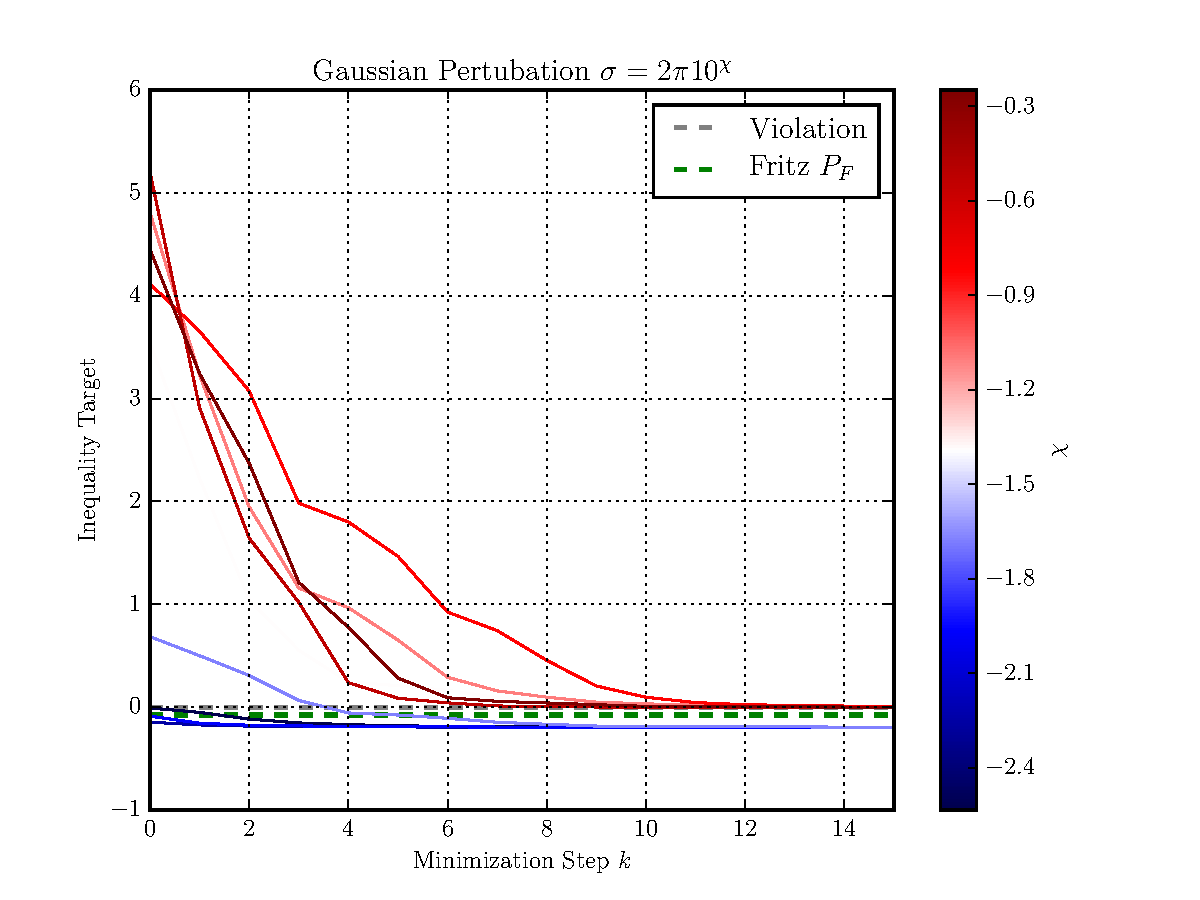
\includegraphics[width=\linewidth]{../../figures/optimizations/Gaussian_Perturbation_Fritz_Color_Default.pdf}}
    % \caption{For each iteration step $k$, the inequality target decreases.}\label{fig:initial_conditions_a}
    % \end{subfigure}
    % \begin{subfigure}[t]{.48\linewidth}
    % {\centering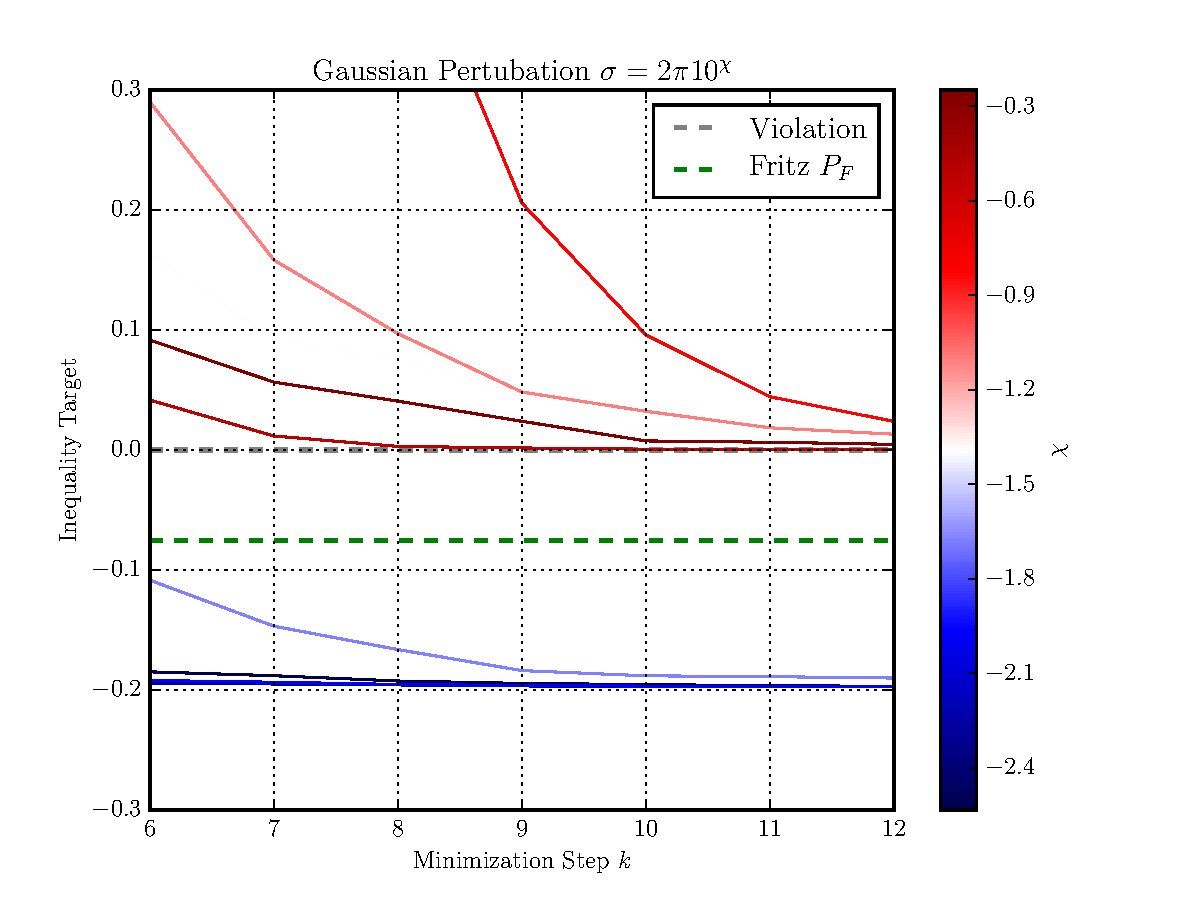
\includegraphics[width=\linewidth]{../../figures/optimizations/Gaussian_Perturbation_Fritz_Color_Zoomed.pdf}}
    % \caption{\Cref{fig:noise} zoomed to show convergence is sensitive to initial conditions.}\label{fig:initial_conditions_b}
    % \end{subfigure}
    % \caption{Numerical optimizations aimed at violating causal compatibility inequalities are sensitive to initial conditions.}\label{fig:initial_conditions}
    % \end{figure}

    The second inequality in consideration is the \textit{symmetric} inequality $I_3$ (\cref{eq:symmetic_web_inequality}). This inequality was able to achieve a greater relative violation than $I_1$ as optimizations converged to a distribution (\cref{fig:maximum_violation_I_3}) with relative violation $V_F \simeq 2.61$. Just as before, the maximum violating distribution shares a possibilistic structure with the Fritz distribution. However, this result is far more surprising. Since the inequality is symmetric with respect to the permutation of parties, one would naively expect that the maximum violating distribution be symmetric as well. If it were not, one could construct a distribution that violates $I_3$ more by symmetrizing $\prob[\fritz]$ by summing over all possible permutations and normalizing. The symmetrized Fritz distribution is plotted in \cref{fig:symmetrized_fritz}. This distribution is also non-classical with relative violation $V_F = 3$. As it turns out, numerical optimizations suggest that the symmetrized Fritz distribution is \textit{not} quantum-accessible in the sense that is cannot be written as \cref{eq:quantum_model_triangle}. Therefore we conclude that the space of quantum accessible correlations on the Triangle structure is non-convex; a reiteration of a result mentioned in~\citet{Inflation}.

    Finally for both $I_0$ and $I_2$, the maximum relative violation happens to be $V_F = 1$ (up to numerical precision). This means that the Fritz distribution either represents a local minimum of the parameter space or is in fact \textit{the} maximally violating distribution. Without further investigations, it remains unclear if this behavior is related to the universality of the Fritz distribution or if its an artifact of the methods used to derive $I_0$ and $I_2$.

    \subsection{Rosset Variation}
    \label{sec:rosset_variation}
    \todo[TC]{This might take a page}


    \section{Conclusions}
    \label{sec:conclusions}
    In \cref{sec:triangle_structure}, we elucidated that compatibility in the Triangle structure has been an unsolved problem for nearly a decade. Initially,~\citet{Branciard_2012} identified the Triangle structure as a challenging causal structure for studying non-classicality. Afterwards,~\citet{Henson_2014} were able to to classify the Triangle structure as \textit{interesting} which partially explains why it remains an enigma. Recently,~\citet{Fritz_2012} discovered the Fritz distribution as the first example of quantum non-classicality in the Triangle structure. In \cref{sec:fritz_distribution} the Fritz distribution was described in detail along with Fritz's Problem~\cite[Problem 2.17]{Fritz_2012}. Heretofore, researchers have been able to derive causal incompatibility inequalities~\cite{Inflation,Steudel_2010,Henson_2014} but unable to show that any are non-trivial in the context of quantum non-classicality.

    In \cref{sec:found_inequalities}, we presented the first examples of causal compatibility inequalities capable of having quantum violations in the sense that they are violated by quantum accessible distributions. This result was made possible through extensive use of the Inflation Technique (\cref{sec:inflation_technique}) when applied to the Fritz distribution. In the context of Fritz's Problem, our result corresponds to a resolution to the following refinement of Fritz's original Problem.
    \begin{enumerate}[label=\textbf{R.\arabic*}]
        \setcounter{enumi}{0}
        \item \label{r:1} Find proofs for causal incompatibility of quantum distributions on the Triangle structure that are \textit{not} reliant on perfect correlations.
    \end{enumerate}

    Ultimately, this work accomplishes two important tasks. First and foremost, the derivation of inequalities such as \cref{eq:ww_ineq} demonstrates the utility of the Inflation Technique specifically for quantum causal inference problems. The Inflation Technique was able to derive causal compatibility inequalities that admit quantum violations in the Triangle structure --- a task that no other existing techniques have succeeded at. In this sense, the results of \cref{sec:found_inequalities} showcase how the Inflation Technique is capable of generating new proofs of causal incompatibility specifically of quantum distributions for the Triangle structure. Consequently, this work strongly indicates that the Inflation Technique has the potential to solve a assortment of unsolved causal inference problems including those manifest in quantum foundations and quantum information theory. Secondly, \cref{sec:noise} demonstrates that the derived causal compatibility inequalities are robust to varying degrees of noise, directly revealing a critical departure from Fritz's original proof of the incompatibility of the Fritz's distribution (\cref{sec:fritz_distribution}) which relies on perfect (non-noisy) correlations. In conclusion \ref{r:1} has been positively solved through the derivation of the inequalities found in \cref{sec:found_inequalities}.

    In consideration of our resolution to \ref{r:1}, we additionally propose two more refinements to Fritz's Problem that are concerned more with the nature of the entanglement resource being exploited in a incompatible quantum distribution:
    \begin{enumerate}[label=\textbf{R.\arabic*}]
        \setcounter{enumi}{1}
        \item \label{r:2} Find incompatible quantum distributions on the Triangle structure that require entanglement in more than one shared state.
        \item \label{r:3} Find incompatible quantum distributions on the Triangle structure that satisfy all Bell structure inequalities under Fritz-type embeddings.
    \end{enumerate}

    Fritz's Problem is concerned with identifying incompatible quantum distributions in the Triangle structure that are qualitatively different than the non-classical distributions of the Bell structure discussed in \cref{sec:bell_structure}. When specifically concerned with entanglement resources, Bell structure non-classicality exploits the entanglement of a single bipartite quantum state. In the Triangle structure, the observable nodes $A,B,C$ have access to potentially three different bipartite quantum states. As noted in \cref{sec:fritz_distribution}, the Fritz distribution can be implemented using only a single entangled state\footnote{Of course there exists implementations that make use of three entangled states but at minimum only one is necessary.}. The question, as proposed by \ref{r:2}, remains: does there exist incompatible quantum distributions that genuinely require the entanglement resources of three states? At first, one might suspect that finding such distributions would affirmatively demonstrate a new form of entanglement resource distinct to the Triangle structure. Unfortunately, this is simply not the case. By increasing the cardinality of the outcomes for $A, B, C$, it is possible to generate a distribution that is non-classical yet quantum and requires all three of the shared resources to be entangled. This can be accomplished by superimposing three copies of statistically independent Fritz distributions to the Triangle Structure, each of which utilizes a distinct party to announce the corresponding measurement pseudo-settings. Such a distribution would be of the form described by \ref{r:2} because under this construction, the removal of any entangled resource would render the distribution quantum-inaccessible.\footnote{This insight was originally made by Miguel Navascués in private communications.} Consequently, it becomes desirable to find non-classical quantum correlations for the Triangle Structure which have the fewest number of outcomes.

    Moreover \ref{r:3} is justified as a valid interpretation of Fritz's Problem in the following sense: the Fritz distribution was constructed by embedding a quantum distribution incompatible with the Bell structure (\cref{fig:bell_scenario}) into the Triangle structure via the re-imagined version of the Triangle scenario (\cref{fig:triangle_structure_with_fritz_bell_embedded}). Furthermore, the logic of \cref{sec:fritz_distribution} shows that \textit{any} Bell structure compatibility inequality can be upgraded to a compatibility inequality for the Triangle structure, provided one restricts the domain of those inequalities to distributions possessing appropriate perfect correlations. Suppose one relaxed that restriction, then it becomes qualitatively reasonable to associate incompatibility via violations of upgraded inequalities with the same variety of incompatibility that is familiar in the Bell structure. Therefore, satisfying all such upgraded inequalities is a sufficient condition for a new type of incompatibility that is genuinely distinct from Bell structure incompatibility. Ultimately, it remains unclear whether or not a positive resolution to \ref{r:3} is even feasible.


    \begin{acknowledgments}
    This research was supported in part by Perimeter Institute for Theoretical Physics. Research at Perimeter Institute is supported by the Government of Canada through the Department of Innovation, Science and Economic Development Canada and by the Province of Ontario through the Ministry of Research, Innovation and Science.
    \end{acknowledgments}

    \appendix

    \section{Summary of Inflation Technique}
    \label{sec:inflation_technique}

    \subsection{Satisfaction of d-Separation Relations}
    \label{sec:satisfaction_of_d_sep_relations}
    \todo[TC]{Absorb the relevant components of the next section into this one}
    \todo[TC]{Given a distribution and a causal structure, does the distribution satisfy the conditional d-Separation relations?}

    \subsection{Marginal Satisfiability and Inequalities}
    \label{sec:marginal_satisfiability}
    \label{sec:marginal_linear}\label{sec:linear_programs}

    This section aims to explain how to solve the following decision problem: given a collection of probability distributions $\bc{\prob[V_1], \ldots, \prob[V_m]}$ where each set of variables $V_{i} \subseteq \jointvar$ is a subset of some complete set of variables $\jointvar$, does there exist a joint distribution $\prob[\jointvar]$ such that each $\prob[V_i]$ can be obtained by marginalizing $\prob[\jointvar]$ over the variables not in $V_i$, i.e. $\prob[V_i] = \sum_{\jointvar \setminus V_i} \prob[\jointvar]$? Colloquially, this problem is referred to as \term{the marginal problem}~\cite{Fritz_2011}. Additionally, this section aims to accomplish something further. If such as joint distribution $\prob[\jointvar]$ exists, how does one find it? Moreover, if a joint distribution does not exist, find an inequality that $\bc{\prob[V_1], \ldots, \prob[V_m]}$ fails which proves such a joint distribution does not exist. This is accomplished by illustrating how the marginal problem can be expressed as a linear program in which the solution to the marginal problem is encoded in the feasibility or infeasibility of said linear program. This section is presented prior to \cref{sec:inflation_technique_main_summary} as the marginal problem becomes an integral component of the Inflation Technique in subsequently deriving the inequalities presented in \cref{sec:found_inequalities}. Moreover, the Marginal problem is presented here logically independent from the remainder of the manuscript both for procedural clarity and because the marginal problem has applications to numerous areas of mathematics including game theory~\cite{Vorobev_1962}, database theory, knowledge integration of expert system, and of course, quantum information theory~\cite{Fritz_2011}.

    To begin, several pieces of nomenclature will be introduced to facilitate discussions. First, the set $\mscenario = \bc{V \mid V \subseteq \jointvar}$ of subsets of $\jointvar$ is referred to as the \term{marginal scenario} and each element $V \in \mscenario$ is termed a \term{(marginal) context} of $\mscenario$. The complete set of marginal distributions is referred to as the \term{marginal model} and is denoted with an superscript $\prob^{\mscenario} \defined \bc{\prob[V] \mid V \in \mscenario}$. A marginal model acts as the most general description of a family of observations that can be made over $\jointvar$. Strictly speaking, as defined by~\cite{Fritz_2011}, a marginal scenario forms an \textit{abstract simplicial complex} where it is required that all subsets of contexts are also contexts: $\forall V \in \mscenario, V' \subset V : V' \in \mscenario$. Throughout this section, we exclusively consider (without loss of generality) the \textit{maximal} marginal scenario; restricting our focus to the largest contexts in the marginal scenario. Additionally, all marginal scenarios are taken to be \text{complete} in the sense that the marginal scenario covers the complete set of observable variables, i.e $\jointvar = \bigcup_{V \in \mscenario} V$. Finally, we henceforth assume that each variable $v \in \s J$ has a finite cardinality.

    The marginal problem asks: given a marginal model $\prob^{\mscenario} = \bc{\prob[V] \mid V \in \mscenario}$ marginal to the joint variables $\jointvar$, does there exist a joint distribution $\prob[\jointvar]$ such that each context $\prob[V]$ can be obtained by marginalizing $\prob[\jointvar]$?
    \[ \forall V \in \mscenario : \prob[V] = \sum_{\jointvar \setminus V} \prob[\jointvar] \eq \label{eq:def:marginal_problem}\]
    A marginal model $\prob^{\mscenario}$ is said to be \textit{contextual} if it \textit{does not} admit a joint distribution and \textit{non-contextual} otherwise. Notice that \cref{eq:def:marginal_problem} is inherently a linear system of constraints which be solved rather efficiently using linear programs. In consideration of this, we will now endeavor to discuss how to cast the \cref{eq:def:marginal_problem} as a matrix multiplication equation so that it becomes possible to discuss existing methods for deriving constraints on the set of contextual marginal models.

    To every discrete random variable $v$ there corresponds a prescribed set of \term{outcomes} $O_v$. We also define the set of all \term{events over $v$}, denoted $\Events{v}$,\footnote{In the language of sheaf-theory, $\Events{v}$ is the \textit{sheaf of events}~\cite{Abramsky_2011}.} to be the set of all functions $s : \bc{v} \to O_v$ each representing the event that a measurement on $v$ was made where $s\br{v} \in O_v$ was observed. Evidently, $\Events{v}$ and $O_v$ have a one-to-one correspondence and this distinction can be confounding. There is rarely any harm in referring synonymously to either as outcomes. Nonetheless, a sheaf-theoretic treatment of contextuality~\cite{Abramsky_2011} demands the distinction.
    Specifically for this work, the distinction becomes essential for our discussion and exploit of marginal symmetries in \cref{sec:symmetric_inequalities}. As a natural generalization we define the events over a set of random variables $V = \bc{v_1, \ldots, v_n}$ in a parallel manner,
    \[ \Events{V} \defined \bc{s: V \to O_{V} \mid \forall i : s\br{v_i} \in O_{v_i} } \eq \label{eq:outcome_space}\]
    Each event $s$ can be compactly represented as a set of mappings over each element of $V$, i.e. $s = \bc{v_i\mapsto s\br{v_i}}_{i = 1}^{k}$. The domain $\Dom{s}$ of an event $s$ is the set of random variables it valuates, i.e. if $s \in \Events{V}$, then $\Dom{s} = V$. Under this framework, a probability distribution $\prob[V]$ can be considered as a map from $\Events{V}$ to the unit interval $\bs{0,1}$.
    The marginal problem inherently depends on the concept of probabilistic marginalization. This concept can be understood at the level of events; one event $s \in \Events{V}$ can be ``marginalized'' or restricted to a smaller event $s' \in \Events{W}$ whenever $W \subseteq V$. For every $W \subseteq V$ and $s \in \Events{V}$, the \term{restriction of $s$ onto $W$} (denoted $s|_{W} \in \Events{W}$) is the event in $\Events{W}$ that \textit{agrees} with each of $s$'s assignments for variables in $W$: $\forall v \in W : s|_{W}\br{v} = s\br{v}$.

    For every marginal scenario $\mscenario = \bc{V_1, \ldots, V_k}$, it is useful to put special emphasis on the \term{joint events} $\Events{\jointvar}$ which represent all possible global events over the entire set of joint variables. Similarly, we define the \term{context events} for a particular context $V \in \mscenario$ as $\Events{V}$. Finally, we elect to define the \term{marginal events} as the disjoint union over all context events and by an abuse of notation we will denote this union as $\Events{\mscenario} = \coprod_{V \in \mscenario} \Events{V}$. Each marginal section $m \in \Events{\mscenario}$ has a domain $\Dom{m} = V$ for some $V \in \mscenario$. By construction each marginal event $m \in \Events{\mscenario}$ is a restriction of some joint event $j \in \Events{\jointvar}$.
    % \subsubsection{Linear Programs}
    % \label{sec:linear_programs}

    The marginalization operation (\cref{eq:def:marginal_problem}) of the marginal problem is a linear operator. This linear operator maps a joint probability distribution $\prob[\jointvar] : \Events{\jointvar} \to \bs{0,1}$ into a marginal model $\prob^{\mscenario} = \bc{\prob[V] : \Events{V} \to \bs{0,1} \mid V \in \mscenario}$. Since $\Events{\mscenario}$ and $\Events{\jointvar}$ are finite, the marginal problem can be represented as a $\abs{\Events{\mscenario}} \times \abs{\Events{\jointvar}}$ matrix.

    \begin{definition}
        \label{def:incidence_matrix}
        The \term{incidence matrix} $M$ for a marginal scenario $\mscenario = \bc{V_1, \dots, V_k}$ is a bit-wise matrix where the columns are indexed by \textit{joint} events $j \in \Events{\jointvar}$ and the rows are events by \textit{marginal} events $m \in \Events{\mscenario}$. The entries of $M$ are populated whenever a marginal event $m$ is a restriction of the joint event $j$.
        \[ M_{m,j} \defined \begin{cases}
            1 & m = j|_{\s{D}\br{m}} \\
            0 & \text{otherwise}
        \end{cases} \]
        The incidence matrix has $\abs{\Events{\jointvar}}$ columns, $\abs{\Events{\mscenario}} = \sum_{i} \abs{\Events{V_i}}$ rows and $k\abs{\Events{\jointvar}}$ non-zero entries.
    \end{definition}
    To illustrate this concretely, consider the following example. Let $\jointvar$ be $3$ binary variables $\jointvar = \bc{A,B,C}$ and $\mscenario$ be the marginal scenario $\mscenario = \bc{\bc{A,B}, \bc{B,C}, \bc{A,C}}$. The incidence matrix for $\mscenario$ is:
    \[ M = \kbordermatrix{
        (A,B,C) \:\: \mapsto & (0,0,0) & (0,0,1) & (0,1,0) & (0,1,1) & (1,0,0) & (1,0,1) & (1,1,0) & (1,1,1) \\
        (A\mapsto0, B\mapsto0) & \kone & \kone & \kzer & \kzer & \kzer & \kzer & \kzer & \kzer \\
        (A\mapsto0, B\mapsto1) & \kzer & \kzer & \kone & \kone & \kzer & \kzer & \kzer & \kzer \\
        (A\mapsto1, B\mapsto0) & \kzer & \kzer & \kzer & \kzer & \kone & \kone & \kzer & \kzer \\
        (A\mapsto1, B\mapsto1) & \kzer & \kzer & \kzer & \kzer & \kzer & \kzer & \kone & \kone \\
        (B\mapsto0, C\mapsto0) & \kone & \kzer & \kzer & \kzer & \kone & \kzer & \kzer & \kzer \\
        (B\mapsto0, C\mapsto1) & \kzer & \kone & \kzer & \kzer & \kzer & \kone & \kzer & \kzer \\
        (B\mapsto1, C\mapsto0) & \kzer & \kzer & \kone & \kzer & \kzer & \kzer & \kone & \kzer \\
        (B\mapsto1, C\mapsto1) & \kzer & \kzer & \kzer & \kone & \kzer & \kzer & \kzer & \kone \\
        (A\mapsto0, C\mapsto0) & \kone & \kzer & \kone & \kzer & \kzer & \kzer & \kzer & \kzer \\
        (A\mapsto0, C\mapsto1) & \kzer & \kone & \kzer & \kone & \kzer & \kzer & \kzer & \kzer \\
        (A\mapsto1, C\mapsto0) & \kzer & \kzer & \kzer & \kzer & \kone & \kzer & \kone & \kzer \\
        (A\mapsto1, C\mapsto1) & \kzer & \kzer & \kzer & \kzer & \kzer & \kone & \kzer & \kone
    } \eq \label{eq:example_incidence}\]
    The incidence matrix needs to act (to the right) on a vector representing the joint probability $\prob[\jointvar]$ distribution and outputs a vector representing the marginal model $\prob^{\mscenario}$. The \term{joint distribution vector} $\probvec^{\jointvar}$ for a probability distribution $\prob[\jointvar]$ is the vector indexed by joint events $j \in \Events{\jointvar}$ whose entries are populated by the probabilities that $\prob[\jointvar]$ assigns to each joint event: $\probvec^{\jointvar}_j = \prob[\jointvar][j]$. Analogously, \term{marginal distribution vector} $\probvec^{\mscenario}$ for a marginal model $\prob^{\mscenario}$ is the vector whose entries are probabilities over the set of marginal outcomes $\Events{\mscenario}$: $\probvec^{\mscenario}_m = \prob[\Dom{m}][m]$.

    By design, the marginal and joint distribution vectors are related via the incidence matrix $M$. Given a joint distribution vector $\probvec^{\jointvar}$ one can obtain the marginal distribution vector $\probvec^{\mscenario}$ by multiplying $M$ by $\probvec^{\jointvar}$.
    \[ \probvec^{\mscenario} = M \cdot \probvec^{\jointvar} \eq \label{eq:incidence_matrix_use} \]
    As a quick remark, the particular ordering of the rows and columns of $M$ carries \textit{no importance}, but it \textit{must} be consistent between $M$, $\probvec^{\jointvar}$ and $\probvec^{\mscenario}$. The marginal problem can now be rephrased in the language of the incidence matrix. Suppose one obtains a marginal distribution vector $\probvec^{\mscenario}$; the marginal problem becomes equivalent to the question: does there exist a joint distribution vector $\probvec^{\jointvar}$ such that \cref{eq:incidence_matrix_use} holds? This question is naturally framed as the \term{marginal linear program}:
    \begin{alignat*}{2}
        & \text{minimize:} \quad&& \emptyset \cdot x\\
        & \text{subject to:} && x \succeq 0 \\
        & && M \cdot x = \probvec^{\mscenario}
    \end{alignat*}
    If this ``optimization''\footnote{``Optimization'' is presented in quotes here because the minimization objective is trivially always zero ($\emptyset$ denotes the null vector of all zero entries). The primal value of the linear program is of no interest, all that matters is its \textit{feasibility}.} is \textit{feasible}, then there exists a vector $x$ than can satisfy \cref{eq:incidence_matrix_use} and is a valid joint distribution vector. Therefore, feasibility of the marginal linear program not only implies that $\probvec^{\jointvar}$ exists but returns $\probvec^{\jointvar}$. Moreover if the marginal linear program is \textit{infeasible}, then there \textit{does not} exist a joint distribution $\probvec^{\jointvar}$. To every linear program, there exists a dual linear program that characterizes the feasibility of the original~\cite{Schrijver_1998}. Constructing the dual linear program is straightforward~\cite{Lahaie_2008}.
    \begin{alignat*}{2}
        & \text{minimize:} \quad&& y \cdot \probvec^{\mscenario}\\
        & \text{subject to:} && y \cdot M \succeq 0
    \end{alignat*}

    The dual marginal linear program not only answers the marginal problem for a specific marginal model $\probvec^{\mscenario}$ but as a by-product provides an inequality that witnesses its contextuality. If this is not obvious, first notice that the dual problem is \textit{never infeasible}; by choosing $y$ to be trivially the null vector $\emptyset$ of appropriate size, all constraints become satisfied. Secondly if the dual constraint $y \cdot M \succeq 0$ holds \textit{and} the primal is feasible, then $y \cdot \probvec^{\mscenario} =  y \cdot M \cdot x \geq 0$. Therefore the \textit{sign} of the dual objective $d \defined \min \br{y \cdot \probvec^{\mscenario}}$ classifies a marginal model's contextuality; if $d < 0$ then $y \cdot \probvec^{\mscenario} \geq 0$ is violated and therefore $\probvec^{\mscenario}$ is contextual. Likewise if $d \geq 0$ (satisfying $y \cdot \probvec^{\mscenario}$), then $\probvec^{\mscenario}$ is non-contextual.\footnote{Actually, if $d \geq 0$ then it is exactly $d = 0$ due to the existence of the trivial $y = \emptyset$. This observation is an instance of the \textit{Complementary Slackness Property} of~\cite{Bradley_1977}. Moreover, if $d < 0$, then it is unbounded $d = -\inf$. This latter point becomes clear upon recognizing that for any $y$ with $d < 0$, another $y' = \al y$ can be constructed (with $\al > 1$) such that $d' = \al d < d$. Since a more negative $d'$ can always be found, it must be that $d$ is unbounded. This is a demonstration of the fundamental \textit{Unboundedness Property} of~\cite{Bradley_1977}; if the dual is unbounded, then the primal is infeasible.} This is manifestation of Farkas's lemma~\cite{Schrijver_1998}. An \term{infeasibility certificate}~\cite{Andersen_2001} is any vector $y$ that satisfies the $y \cdot M \succeq 0$. Most linear program software packages such as Mosek~\cite{Mosek_2016}, Gurobi~\cite{Gurobi_2016}, CPLEX~\cite{Cplex_2016} and CVX/CVX OPT~\cite{CVX_2016,CVX_Opt_2016} are capable of producing infeasibility certificates. Furthermore, for every $y$ satisfying $y \cdot M \succeq 0$ there corresponds a \term{certificate inequality} that constraints the set of non-contextual marginal models. If $y$ is an infeasibility certificate, then $y \cdot \probvec^{\mscenario} \geq 0$ is satisfied by all contextual marginal models.

    The marginal problem can sometimes take on a more general variant that does not begin with a specific marginal model~\cite{Abramsky_2012,Mansfield_2012,Fritz_2011}: \textit{Given a marginal scenario $\mscenario$, what is the set of all non-contextual marginal models?} \citet{Pitowsky_1991} demonstrates that the set of non-contextual marginal models forms a \textit{convex} polytope called the \term{marginal polytope}. The extremal rays of a marginal polytope directly correspond to the columns of $M$ which further correspond to \textit{deterministic} joint distributions $\probvec^{\jointvar}$. Since all joint distributions $\probvec^{\jointvar}$ are probability distributions, their entries must sum to unity $\sum_{j \in \Events{\jointvar}} \probvec^{\jointvar}_j = 1$. This normalization defines the convexity of the polytope; all non-contextual marginal models are convex mixtures of the deterministic marginal models pursuant to \cref{eq:incidence_matrix_use}. The marginal polytope is a beneficial tool for understanding contextuality. First, the \textit{facets} of a marginal polytope correspond to a finite set of linear inequalities that are complete in the sense that all contextual distributions violate at least one facet inequality~\cite{Brunner_2013}. From the perspective of a marginal polytope, convex hull algorithms or linear quantifier elimination can be used to compute a representation of the complete set of linear inequalities and completely solve the marginal problem. A popular tool for linear quantifier elimination is \term{Fourier-Motzkin elimination} \cite{Dantzig_1973,Inflation,Abramsky_2012,jones_2004}. Applying the Fourier-Motzkin procedure to completely solve the marginal problem is discussed in more detail in \citet{Fritz_2011}. An excellent survey of existing techniques for solving the marginal problem including Equality Set Projection~\cite{jones_2004} and Hardy-type hypergraph transversals can be found in \citet{Inflation}. In conclusion, there are a number of computational tools available to solve the marginal problem completely whenever no marginal model is provided.

    Each of the above mentioned techniques suffers from computational complexity limitations. For example, the Fourier-Motzkin procedure is in the worst case doubly exponential in the number of initial inequalities~\cite{Dantzig_1973}. For the purposes of this research, solving the marginal problem without reference to a marginal model was intractable. This will become apparent in \cref{sec:exemplary_inflations_of_the_triangle structure} when the Inflation Technique is applied to the Triangle structure, producing marginal models that are very large. Luckily, the Fritz distribution (\cref{sec:fritz_distribution}) allows one to avoid the complexity issues of the complete marginal problem and instead focus on the original problem of determining whether or not a particular marginal model admits a joint distribution or not.
    \subsection{Inflation Technique}
    \label{sec:deriving_inequalities}
    \label{sec:inflation_technique_main_summary}
    The \term{Inflation Technique}, invented by \citet{Inflation} and inspired by the \textit{do calculus} and \textit{twin networks} of \citet{Pearl_2009}, is a family of causal inference techniques that can be used to determine if probability distribution $\prob[\nodes_{O}]$ is compatible or incompatible with a given causal structure $\graph$. As a preliminary summary, the Inflation Technique begins by \textit{augmenting} a causal structure with additional copies of its nodes, producing an \textit{inflated} causal structure, and then exposes how causal inference tasks on the inflated causal structure can be used to make inferences on the original causal structure. As a example, four inflations of the Triangle structure are depicted in \cref{fig:inflations}. Copies of nodes in the inflated causal structure are distinguished by an additional subscript called the \term{copy-index}. For example, node $A$ of \cref{fig:triangle_structure} has copies $A_1, A_2, A_3, A_4$ in the inflated causal structure in \cref{fig:the_web_inflation}. All such copies are deemed equivalent via a \term{copy-index equivalence} relation denoted `$\sim$'. A copy-index is effectively arbitrary, so we will refer to an arbitrary inflated copy of $A$ as $A'$.
    \[ A \sim A_1 \sim A' \not\sim B \sim B_1 \sim B' \]
    We preemptively generalize the notion of copy-index equivalence to other mathematical objects like sets, graphs, and groups by saying that $X \sim Y$ if and only if $X = Y$ upon removal of the copy-index. In addition to the common graph-theoretic terminology and notation presented in \cref{sec:causal_compatibility}, we define two more concepts necessary to formally define an inflation of $\graph$. First, an \term{induced subgraph} of $\graph$ for a subset of nodes $N \subseteq \nodes$ is another graph composed of nodes $N$ and all edges $e$ of the original graph that are contained in $N$: $\Sub[\graph]{N} \defined \br{N, \bc{e = \bc{n \to m} \mid n, m \in N}}$. An \term{ancestral subgraph} of $\graph$ for a subset of nodes $N \subseteq \nodes$ is the induced subgraph due to the ancestry of $N$: $\AnSub[\graph]{N} \defined \Sub[\graph]{\An[\graph]{N}}$.

    \begin{definition}
        An \term{inflation} of a causal structure $\graph$ is another causal structure $\graph'$ such that:
        \[ \forall n' \in \nodes': \AnSub[\graph']{n'} \sim \AnSub[\graph]{n} \eq \label{eq:inflation_defn}\]
    \end{definition}
    Verbally, for each inflated node $n'$, the ancestral sub-graph of $n'$ in $\graph'$ is equivalent to its counterpart in $\graph$ up to copy-index. The motivation behind this definition is that if the ancestry of each node $n'$ in $\graph'$ plays the \textit{exact same} role as the ancestry of its source copy $n$ in $\graph$, then every compatible distribution $\prob[N]$ on $\graph$ can be used to \textit{create} compatible joint distributions on $\graph'$. To do this, first notice that for every distribution $\prob[N]$ compatible with $\graph$, there must exist a set of causal parameters $\{\prob[n\mid \Pa[\graph]{n}] \mid n \in \nodes\}$ for $\graph$ such that $\prob[N] = \prod_{n \in N} \prob[n\mid \Pa[\graph]{n}]$. Since the inflation criteria (\cref{eq:inflation_defn}) requires that $\Pa[\graph']{n'} \sim \Pa[\graph]{n}$ one can create a set of \term{inflated causal parameters} by matching causal parameters according to respective copy-indices.
    \[ \forall n' \in \nodes' : \prob[n'\mid \Pa[\graph']{n'}] \defined \prob[n\mid \Pa[\graph]{n}] \eq \label{eq:inflated_causal_parameters} \]
    Which in turn uniquely defines a compatible joint distribution $\prob[\nodes']$ on $\graph'$\footnote{Of course, there exists compatible joint distributions on $\nodes'$ that can not be constructed in this manner. The claim is that all joint distributions that are constructed in this way are compatible.}.
    \[ \prob[\nodes'] = \prod_{n' \in \nodes'} \prob[n'\mid \Pa[\graph']{n'}] \eq \label{eq:unique_causal_parameters_inflated}\]
    % \cref{eq:unique_causal_parameters,eq:inflated_causal_parameters,eq:unique_causal_parameters_inflated}
    Together, ??  form the \term{weak inflation lemma}: compatible joint distributions over $\nodes$ induce compatible joint distributions over $\nodes'$. Before generalizing to the inflation lemma, a careful observation needs to be made. For any pair of subsets of nodes $N \subseteq \nodes$ and $N' \subseteq \nodes'$ that are equivalent up to copy-index $N \sim N'$, if $\AnSub[\graph]{N} \sim \AnSub[\graph']{N'}$ then any compatible \textit{marginal} distribution $\prob[N]$, where $N \subset \nodes$, induces a compatible marginal distribution $\prob[N']$ over $N'$. In fact, $N'$ must contain no duplicate nodes up to copy index and thus $\prob[N] = \prob[N']$. These subsets of nodes are so essential to the Inflation Technique they are assigned a special name: sets $N' \subseteq \nodes'$ as called the \term{injectable sets} of $\graph'$ and $N \subset \nodes$ the \term{images of the injectable sets} of $\graph$.
    \begin{align*}
        \Inj[\graph]{\graph'} &\defined \bc{N' \subseteq \nodes' \mid \exists N \subseteq \nodes : N \sim N'} \\
        \ImInj[\graph]{\graph'} &\defined \bc{N \subseteq \nodes \mid \exists N' \subseteq \nodes' : N \sim N'}
    \end{align*}
    Injectable sets are incredibly useful for causal compatibility because they allow one to extend the weak inflation lemma to \textit{the} inflation lemma:
    \todo[TC]{How do I claim the inflation lemma without defining compatibility over a marginal model (instead of a distribution)}
    \begin{lemma}
        \label[lemma]{lem:inflation}
        \term{The Inflation Lemma}~\cite[Lemma 3]{Inflation} Given a particular inflation $\graph'$ of $\graph$ and a marginal model $\bc{\prob[N] \mid N \in \ImInj[\graph]{\graph'}}$ compatible with $\graph$ then all marginal models $\bc{\prob[N'] \mid N' \in \Inj[\graph]{\graph'}}$ are compatible with $\graph'$ provided that $\prob[N] = \prob[N']$ for all instances where $N \sim N'$.
    \end{lemma}
    Diagrammatically, \cref{lem:inflation} can be visualized as follows:

    \begin{center}
        \begin{tikzpicture}
            \pgfmathsetmacro{\vs}{2.2};
            \pgfmathsetmacro{\hs}{5.2};
            \draw (0*\hs,0*\vs) node[](pn){$\underbrace{\bc{\prob[N] \mid N \in \ImInj[\graph]{\graph'}}}_{\text{compatible with $\graph$}}$};
            \draw (1*\hs,0*\vs) node[](cp){$\bc{\prob[n\mid \Pa[\graph]{n}] \mid n \in \nodes}$};
            \draw (1*\hs,-1*\vs) node[](cp_){$\bc{\prob[n'\mid \Pa[\graph']{n'}] \mid n' \in \nodes'}$};
            \draw (0*\hs,-1*\vs) node[](pn_){$\underbrace{\bc{\prob[N'] \mid N' \in \Inj[\graph]{\graph'}}}_{\text{compatible with $\graph'$}}$};
            \draw[very thick, ->] (pn) -- (cp);
            \draw[very thick, ->] (cp) -- (cp_) node [midway, above, sloped]{{\footnotesize define}};
            \draw[very thick, ->] (cp_) -- (pn_);
        \end{tikzpicture}
    \end{center}

    The inflation lemma is the most important result of the causal Inflation Technique. The contrapositive version of \cref{lem:inflation} is a powerful tool for deriving causal compatibility constraints. Any causal compatibility constraint, such as a causal compatibility inequality, that constrains injectable marginal models $\bc{\prob[N'] \mid N' \in \Inj[\graph]{\graph'}}$ can be \textit{deflated} into a valid compatibility constraint on marginal models $\bc{\prob[N] \mid N \in \ImInj[\graph]{\graph'}}$ of the original causal structure by dropping all references to the copy-indices. Additionally, the inflation lemma holds when considering any subset of $\Inj[\graph]{\graph'}$ (analogously $\ImInj[\graph]{\graph'}$). Therefore, one only needs to consider injectable sets that are composed of \textit{observable nodes}.

    Heretofore, the Inflation Technique as stated by \cref{lem:inflation} does not facilitate the derivation of any non-trivial inequalities. The Inflation lemma simply casts causal inference problems on $\graph$ to causal inference problems on $\graph'$. Fortunately, an inflated causal structure $\graph'$ possesses its own conditional independence relations which can be exploited to turn linear inequalities on $\graph'$ into polynomial inequalities on $\graph$.

    Suppose that one were to obtain an inequality on $\graph'$ that contained probabilistic terms such as $\prob[N']$ where $N' \not \in \Inj[\graph]{\graph'}$. At this point, the Inflation lemma is not applicable because it requires probabilistic constraints to consist entirely of distributions $\prob[N']$ where $N'$ is injectable. If for example, $N' \not \in \Inj[\graph]{\graph'}$ could be partitioned into two injectable subsets $N_1' \in \Inj[\graph]{\graph'}$ and $N_2' \in \Inj[\graph]{\graph'}$ that where \term{ancestrally independent} in $\graph'$,
    \[ N_1' \ancestralindep N_2' \iff \An[\graph']{N_1'} \cap \An[\graph']{N_2'}= \emptyset \]
    Then the compatible marginal context $\prob[N']$ must be probabilistically separable $\prob[N'] = \prob[N_1']\prob[N_2']$ due to \cref{eq:local_markov_property}. Since $N_1'$ and $N_2'$ are both injectable, the inflation lemma now applies and the original inequality can be deflated.

    \begin{center}
        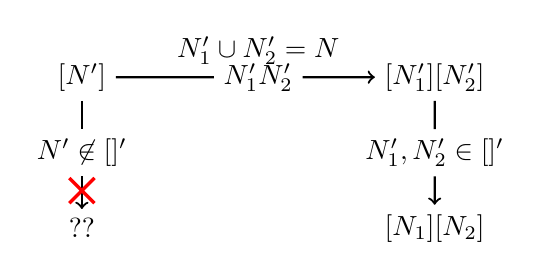
\begin{tikzpicture}[scale=0.8]
            \pgfmathsetmacro{\hs}{1.4};
            \pgfmathsetmacro{\vs}{0.6};
            \pgfmathsetmacro{\cross}{0.2};
            \draw (0*\hs, 4*\vs) node[](a){$\prob[N']$};
            \draw (0*\hs, 2*\vs) node[](ab){$N' \not \in \Inj[\graph]{\graph'}$};
            \draw (4*\hs, 4*\vs) node[](c){$\prob[N_1']\prob[N_2']$};
            \draw (2*\hs, 4*\vs) node[](ac){$N_1' \ancestralindep N_2'$};
            \draw (2*\hs, 4*\vs + 0.7*\vs) node[]{$N_1' \cup N_2' = N$};
            \draw (4*\hs, 2*\vs) node[](cd){$N_1', N_2' \in \Inj[\graph]{\graph'}$};
            \draw (4*\hs, 0*\vs) node[](d){$\prob[N_1]\prob[N_2]$};
            \draw (0, 0) node[](b){??};
            \draw[thick, ] (a) -- (ab);
            \draw[thick, ] (c) -- (cd);
            \draw[thick, ] (a) -- (ac);
            \draw[thick, ->] (ac) -- (c);
            \draw[thick, ->] (ab) -- (b);
            \draw[thick, ->] (cd) -- (d);
            \draw[very thick, red]
            (+ \cross, 1*\vs + \cross) -- (- \cross, 1*\vs - \cross)
            (+ \cross, 1*\vs - \cross) -- (- \cross, 1*\vs + \cross)
            ;
        \end{tikzpicture}
    \end{center}

    Not all sets $N' \subseteq \nodes'$ can be written as the disjoint union of injectable sets, but those that can are called the \term{pre-injectable sets}. A set $N' \subseteq \nodes'$ is a pre-injectable set if it can be decomposed into the disjoint union of injectable sets $N' = \coprod_{i} N'_i \mid N'_i \in \Inj[\graph]{\graph'}$ and all pairs $N_i', N_j'$ are ancestrally independent: $\forall i, j : N_i' \ancestralindep N_j'$.

    A pre-injectable set $N'$ is of primal importance to the Inflation Technique because any distribution over $N'$ will factorize according to graphical $d$-separation conditions~\cite{Pearl_2009},
    \[ \prob[N'] = \prob[\coprod_i N'_i] = \prod_{i}\prob[N'_i] \]
    Application of the inflation lemma to linear inequalities constraining pre-injectable distributions $\prob[N']$ transforms those inequalities into polynomial inequalities over the injectable distributions, allowing one to replace all terms with probability distributions defined over variables in $\nodes$. Throughout the body of this work, we let $\PreInj[\graph]{\graph'}$ denote the set of all pre-injectable sets. Naturally, the pre-injectable sets will define a marginal scenario $\mscenario$ that are used to derive compatibility inequalities in \cref{sec:deriving_inequalities}\footnote{Analogously for a marginal scenario $\mscenario$, the pre-injectable sets $\PreInj[\graph]{\graph'}$ form an \textit{abstract simplicial complex}. Therefore, in practice, it is completely sufficient to focus on the maximal pre-injectable sets}.

    \subsection{Exemplary Inflations of The Triangle Structure}
    \label{sec:exemplary_inflations_of_the_triangle structure}

    \Cref{sec:inflation_technique_main_summary} explains how the Inflation Technique~\cite{Inflation} was used to derive novel causal compatibility inequalities for the Triangle Structure by constructing inflations of the Triangle Structure satisfying \cref{eq:inflation_defn}. Explicitly, for a given inflation $\graph'$ of the Triangle Structure, one constructs a marginal problem (see \cref{sec:marginal_satisfiability}) for the marginal scenario $\mscenario$ composed of the maximal pre-injectable sets of $\graph'$, i.e. $\mscenario = \PreInj[\graph]{\graph'}$. This section acts as a reference for the particular inflations of the Triangle scenario that are mentioned throughout this manuscript. Contained within this section is a depiction of each of these inflations in \cref{fig:inflations} as well as a their pre-injectable sets. An efficient algorithm for computing the injectable and pre-injectable sets of an inflation can be found in~\cite{Inflation}.
    \begin{center}
    \begin{figure}
    \begin{subfigure}[b]{.45\linewidth}
    \scalebox{1}{\newcommand{\ift}{2.3}
\begin{tikzpicture}[scale=2]
    \begin{scope}[every node/.style=observed]
        \node (C1) at ({-2 + 3*1/\ift}, {3*1/(\ift*sqrt(3))}) {$\p{C}_1$};
        \node (B1) at ({2 - 3*1/\ift}, {3*1/(\ift*sqrt(3))}) {$\p{B}_1$};
        \node (A1) at (0, {2*sqrt(3) - 2*2/sqrt(3)*(1/\ift)}) {$\p{A}_1$};
    \end{scope}
    \begin{scope}[every node/.style=latent]
        \node (X1) at ({-1 + 1/\ift}, {sqrt(3) - 1/(\ift*sqrt(3))}) {$\p{X}_1$};
        \node (Y2) at (1, {sqrt(3)}) {$\p{Y}_2$};
        \node (Y1) at ({1 - 1/\ift}, {sqrt(3) - 1/(\ift*sqrt(3))}) {$\p{Y}_1$};
        \node (Z1) at (0, 0.5) {$\p{Z}_1$};
    \end{scope}
    \begin{scope}[every path/.style={draw=cause, thick}]
        \path[postaction={on each segment={mid arrow}}]
        (X1) -- (A1) (X1) -- (C1)
        (Y2) -- (A1) (Y1) -- (B1)
        (Z1) -- (B1) (Z1) -- (C1)
        ;
    \end{scope}
\end{tikzpicture}}
    \caption{The Cut inflation.}\label{fig:cut_inflation}
    \end{subfigure}
    \begin{subfigure}[b]{.45\linewidth}
    \scalebox{1}{\newcommand{\ift}{2.3}
\begin{tikzpicture}[scale=2]
    \begin{scope}[every node/.style=observed]
        \node (C2) at ({-2 + 2*1/\ift}, {2*1/(\ift*sqrt(3))}) {$\p{C}_2$};
        \node (C1) at ({-2 + 3*1/\ift}, {3*1/(\ift*sqrt(3))}) {$\p{C}_1$};
        \node (B2) at ({2 - 2*1/\ift}, {2*1/(\ift*sqrt(3))}) {$\p{B}_2$};
        \node (B1) at ({2 - 3*1/\ift}, {3*1/(\ift*sqrt(3))}) {$\p{B}_1$};
        \node (A2) at (0, {2*sqrt(3) - 2*2/sqrt(3)*(1/\ift)}) {$\p{A}_2$};
        \node (A1) at (0, {2*sqrt(3) - 3*2/sqrt(3)*(1/\ift)}) {$\p{A}_1$};
    \end{scope}
    \begin{scope}[every node/.style=latent]
        \node (X2) at (-1, {sqrt(3)}) {$\p{X}_2$};
        \node (X1) at ({-1 + 1/\ift}, {sqrt(3) - 1/(\ift*sqrt(3))}) {$\p{X}_1$};
        \node (Y2) at (1, {sqrt(3)}) {$\p{Y}_2$};
        \node (Y1) at ({1 - 1/\ift}, {sqrt(3) - 1/(\ift*sqrt(3))}) {$\p{Y}_1$};
        \node (Z1) at (0, 0.5) {$\p{Z}_1$};
        \node (Z2) at (0, 0) {$\p{Z}_2$};
    \end{scope}
    \begin{scope}[every path/.style={draw=cause, thick}]
        \path[postaction={on each segment={mid arrow}}]
        (X1) -- (A1) (X1) -- (C1) (X2) -- (C2) (X1) -- (A2)
        (Y1) -- (A1) (Y1) -- (B1) (Y2) -- (A2) (Y1) -- (B2)
        (Z1) -- (B1) (Z1) -- (C1) (Z2) -- (B2) (Z1) -- (C2)
        ;
    \end{scope}
\end{tikzpicture}}
    \caption{The Spiral inflation.}\label{fig:spiral_inflation}
    \end{subfigure}

    \begin{subfigure}[b]{.45\linewidth}
    \scalebox{1.0}{\newcommand{\ift}{2.3}
\newcommand{\hvspoke}{0.8}
\newcommand{\diagspoke}{1.1}
\begin{tikzpicture}[scale=2]
    \begin{scope}[every node/.style=observed]
        \node (A1) at ({0}, {\hvspoke}) {$\p{A}_1$};
        \node (A2) at ({0}, {-\hvspoke}) {$\p{A}_2$};
        \node (B1) at ({-\hvspoke}, {0}) {$\p{B}_1$};
        \node (B2) at ({\hvspoke}, {0}) {$\p{B}_2$};
        \node (C1) at ({+\diagspoke}, {+\diagspoke}) {$\p{C}_1$};
        \node (C2) at ({+\diagspoke}, {-\diagspoke}) {$\p{C}_2$};
        \node (C3) at ({-\diagspoke}, {-\diagspoke}) {$\p{C}_3$};
        \node (C4) at ({-\diagspoke}, {+\diagspoke}) {$\p{C}_4$};
    \end{scope}
    \begin{scope}[every node/.style=latent]
        \node (Y1) at (0, 0) {$\p{Y}_1$};
        \node (X1) at ({0}, {2*\hvspoke}) {$\p{X}_1$};
        \node (Z1) at ({2*\hvspoke}, {0}) {$\p{Z}_1$};
        \node (X2) at ({0}, {-2*\hvspoke}) {$\p{X}_2$};
        \node (Z2) at ({-2*\hvspoke}, {0}) {$\p{Z}_2$};
    \end{scope}
    \begin{scope}[every path/.style={draw=cause, thick}]
        \path[postaction={on each segment={mid arrow}}]
        % Y1
        (Y1) -- (A1)
        (Y1) -- (A2)
        (Y1) -- (B1)
        (Y1) -- (B2)
        % X1
        (X1) -- (C1)
        (X1) -- (C4)
        (X1) -- (A1)
        % Z1
        (Z1) -- (C1)
        (Z1) -- (C2)
        (Z1) -- (B2)
        % X2
        (X2) -- (C2)
        (X2) -- (C3)
        (X2) -- (A2)
        % Z2
        (Z2) -- (C4)
        (Z2) -- (C3)
        (Z2) -- (B1)
        ;
    \end{scope}
\end{tikzpicture}}
    \caption{The Wagon-Wheel inflation.}\label{fig:wagon_wheel_inflation}
    \end{subfigure}
    \begin{subfigure}[b]{.45\linewidth}
    \scalebox{1}{\newcommand{\ift}{2.3}
\begin{tikzpicture}[scale=2]
    \begin{scope}[every node/.style=observed]
        \node (C4) at (-2, 0) {$\p{C}_4$};
        \node (C3) at ({-2 + 1/\ift}, {1/(\ift*sqrt(3))}) {$\p{C}_3$};
        \node (C2) at ({-2 + 2*1/\ift}, {2*1/(\ift*sqrt(3))}) {$\p{C}_2$};
        \node (C1) at ({-2 + 3*1/\ift}, {3*1/(\ift*sqrt(3))}) {$\p{C}_1$};
        \node (B4) at (2, 0) {$\p{B}_4$};
        \node (B3) at ({2 - 1/\ift}, {1/(\ift*sqrt(3))}) {$\p{B}_3$};
        \node (B2) at ({2 - 2*1/\ift}, {2*1/(\ift*sqrt(3))}) {$\p{B}_2$};
        \node (B1) at ({2 - 3*1/\ift}, {3*1/(\ift*sqrt(3))}) {$\p{B}_1$};
        \node (A4) at (0, {2*sqrt(3)}) {$\p{A}_4$};
        \node (A3) at (0, {2*sqrt(3) - 2/sqrt(3)*(1/\ift)}) {$\p{A}_3$};
        \node (A2) at (0, {2*sqrt(3) - 2*2/sqrt(3)*(1/\ift)}) {$\p{A}_2$};
        \node (A1) at (0, {2*sqrt(3) - 3*2/sqrt(3)*(1/\ift)}) {$\p{A}_1$};
    \end{scope}
    \begin{scope}[every node/.style=latent]
        \node (X2) at (-1, {sqrt(3)}) {$\p{X}_2$};
        \node (X1) at ({-1 + 1/\ift}, {sqrt(3) - 1/(\ift*sqrt(3))}) {$\p{X}_1$};
        \node (Y2) at (1, {sqrt(3)}) {$\p{Y}_2$};
        \node (Y1) at ({1 - 1/\ift}, {sqrt(3) - 1/(\ift*sqrt(3))}) {$\p{Y}_1$};
        \node (Z1) at (0, 0.5) {$\p{Z}_1$};
        \node (Z2) at (0, 0) {$\p{Z}_2$};
    \end{scope}
    \begin{scope}[every path/.style={draw=cause, thick}]
        \path[postaction={on each segment={mid arrow}}]
        (X2) -- (A4) (X2) -- (C4) (X2) -- (C2) (X2) -- (A3)
        (Y2) -- (A4) (Y2) -- (B4) (Y2) -- (A2) (Y2) -- (B3)
        (Z2) -- (B4) (Z2) -- (C4) (Z2) -- (B2) (Z2) -- (C3)
        (X1) -- (A1) (X1) -- (C1) (X1) -- (C3) (X1) -- (A2)
        (Y1) -- (A1) (Y1) -- (B1) (Y1) -- (A3) (Y1) -- (B2)
        (Z1) -- (B1) (Z1) -- (C1) (Z1) -- (B3) (Z1) -- (C2)
        ;
    \end{scope}
\end{tikzpicture}}
    \caption{The Web Inflation.}\label{fig:the_web_inflation}
    \end{subfigure}
    \caption{Some inflations of the Triangle structure.}
    \label{fig:inflations}
    \end{figure}
    \end{center}

    The first inequality presented in \cref{sec:found_inequalities} was \cref{eq:ww_ineq}. \cref{eq:ww_ineq} was derived using the Wagon-Wheel inflation in \cref{fig:wagon_wheel_inflation}. The Wagon-Wheel inflation possesses $4$ copies of $C$ ($C_1, C_2, C_3, C_4$) and $2$ copies of $A$ ($A_1, A_2$) and $B$ ($B_1, B_2$) arranged in the shape of a Wagon-Wheel. The maximal pre-injectable sets of the Wagon-Wheel inflation along with their ancestral dependences can be found in \cref{eq:pre_injectable_triangle_structure_wagon_wheel}. These maximal pre-injectable sets define the following marginal scenario where the joint variables $\jointvar$ are simply the set of observable nodes in the Wagon-Wheel inflation $\jointvar = \nodes'_O$:
    \[ \mscenario = \PreInj[\graph]{\graph'} = \bc{\bc{A_2, B_1, C_3, C_1}, \bc{A_1, B_1, C_4, C_2}, \bc{A_1, B_2, C_1, C_3}, \bc{A_2, B_2, C_2, C_4}} \eq \label{eq:wagon_wheel_marginal_model}\]
    Given that the Fritz distribution is defined over $4$-outcomes variables, the variables in the marginal scenario are assigned $4$-outcomes as well. This marginal scenario $\mscenario$ then defines an incidence matrix $M$ capable of accommodating the Fritz distribution that has $\abs{\Events{\mscenario}} = 4 \cdot 4^{4} = 1024$ rows and $\abs{\Events{\jointvar}} = 4^8 = 65,536$ columns. Understandably, this matrix is not reproduced here. The sheer size of the incidence matrix used here makes complete solutions of the marginal problem using tools such as linear-quantifier elimination intractable.

    \begin{equation*}
        \eq \label{eq:pre_injectable_triangle_structure_wagon_wheel}
        \begin{gathered}
            \textbf{Maximal Pre-injectable Sets} \\
            \bc{A_2, B_1, C_3, C_1} \\
            \bc{A_1, B_1, C_4, C_2} \\
            \bc{A_1, B_2, C_1, C_3} \\
            \bc{A_2, B_2, C_2, C_4} \\
        \end{gathered}
        \qquad
        \begin{gathered}
            \textbf{Ancestral Independences} \\
            \bc{A_2, B_1, C_3} \ancestralindep \bc{C_1} \\
            \bc{A_1, B_1, C_4} \ancestralindep \bc{C_2} \\
            \bc{A_1, B_2, C_1} \ancestralindep \bc{C_3} \\
            \bc{A_2, B_2, C_2} \ancestralindep \bc{C_4} \\
        \end{gathered}
    \end{equation*}
    To construct the marginal distribution vector $\probvec^{\mscenario}$ for the Fritz distribution, one begins with $\probvec^{\mscenario}$ defined in a \textit{symbolic} form,
    \[ {\probvec^{\mscenario}}^{\intercal} = \underbrace{\br{\prob[A_2B_1C_3C_1]\br{0000}, \ldots, \prob[A_1B_1C_4C_2]\br{3232}, \ldots, \prob[A_2B_2C_2C_4]\br{3333}}}_{1024 \text{ entries}} \eq \label{eq:marginal_vector_wagon_wheel} \]
    Which can be factored into the ancestrally independent injectable sets using \cref{eq:pre_injectable_triangle_structure_wagon_wheel},
    \[ {\probvec^{\mscenario}}^{\intercal} = \br{\prob[A_2B_1C_3]\br{000}\prob[C_1]\br{0}, \ldots, \prob[A_1B_1C_4]\br{323}\prob[C_2]\br{2}, \ldots, \prob[A_2B_2C_2]\br{333}\prob[C_4]\br{3}} \eq \label{eq:marginal_vector_wagon_wheel_factors}\]
    And penultimately, each probability distribution in \cref{eq:marginal_vector_wagon_wheel_factors} is deflated by dropping copy-indices.
    \[ {\probvec^{\mscenario}}^{\intercal} = \br{\prob[ABC]\br{000}\prob[C]\br{0}, \ldots, \prob[ABC]\br{323}\prob[C]\br{2}, \ldots, \prob[ABC]\br{333}\prob[C]\br{3}} \eq \label{eq:marginal_vector_wagon_wheel_factors_dropped}\]
    This step is permitted because all of the remaining distributions in \cref{eq:marginal_vector_wagon_wheel_factors} are defined over the injectable sets of the Wagon-Wheel inflation. Finally, each of the elements of $\probvec^{\mscenario}$ are replaced with numerical values pursuant to the Fritz distribution. For example, $\prob[ABC]\br{323}\prob[C]\br{2}$ is assigned the following numerical value:
    \[ \prob[ABC]\br{323}\prob[C]\br{2} = \f{1}{32}\br{2 + \sqrt{2}} \cdot \f{1}{4} \simeq 0.0267  \]
    The same is applied to all other entries of $\probvec^{\mscenario}$. Finally, this numerical version of $\probvec^{\mscenario}$ and $M$ are subjected to linear programing software and an infeasibility certificate $y$ was obtained, corresponding precisely to \cref{eq:ww_ineq} using \cref{eq:marginal_vector_wagon_wheel_factors_dropped}.

    The remaining inequalities in \cref{sec:found_inequalities} were derived using the Web inflation of \cref{fig:the_web_inflation}. The maximal pre-injectable sets of the Wagon-Wheel inflation along with their ancestral dependences can be found in \cref{eq:pre_injectable_triangle_structure_web}.
    \begin{equation*}
        \eq \label{eq:pre_injectable_triangle_structure_web}
        \begin{gathered}
            \textbf{Maximal Pre-injectable Sets} \\
            \bc{A_1, B_1, C_1, A_4, B_4, C_4} \\
            \bc{A_1, B_2, C_3, A_4, B_3, C_2} \\
            \bc{A_2, B_3, C_1, A_3, B_2, C_4} \\
            \bc{A_2, B_4, C_3, A_3, B_1, C_2} \\
            \bc{A_1, B_3, C_4} \\
            \bc{A_1, B_4, C_2} \\
            \bc{A_2, B_1, C_4} \\
            \bc{A_2, B_2, C_2} \\
            \bc{A_3, B_3, C_3} \\
            \bc{A_3, B_4, C_1} \\
            \bc{A_4, B_1, C_3} \\
            \bc{A_4, B_2, C_1}
        \end{gathered}
        \qquad
        \begin{gathered}
            \textbf{Ancestral Independences} \\
            \bc{A_1, B_1, C_1} \ancestralindep \bc{A_4, B_4, C_4} \\
            \bc{A_1, B_2, C_3} \ancestralindep \bc{A_4, B_3, C_2} \\
            \bc{A_2, B_3, C_1} \ancestralindep \bc{A_3, B_2, C_4} \\
            \bc{A_2, B_4, C_3} \ancestralindep \bc{A_3, B_1, C_2} \\
            \bc{A_1} \ancestralindep \bc{B_3} \ancestralindep \bc{C_4} \\
            \bc{A_1} \ancestralindep \bc{B_4} \ancestralindep \bc{C_2} \\
            \bc{A_2} \ancestralindep \bc{B_1} \ancestralindep \bc{C_4} \\
            \bc{A_2} \ancestralindep \bc{B_2} \ancestralindep \bc{C_2} \\
            \bc{A_3} \ancestralindep \bc{B_3} \ancestralindep \bc{C_3} \\
            \bc{A_3} \ancestralindep \bc{B_4} \ancestralindep \bc{C_1} \\
            \bc{A_4} \ancestralindep \bc{B_1} \ancestralindep \bc{C_3} \\
            \bc{A_4} \ancestralindep \bc{B_2} \ancestralindep \bc{C_1}
        \end{gathered}
    \end{equation*}
    Analogously to the Wagon-Wheel inflation, these pre-injectable sets form a marginal scenario $\mscenario$ which defines an incidence matrix $M$ that has $\abs{\Events{\mscenario}} = 4 \cdot 4^{6} + 8 \cdot 4^3 = 16,896$ rows, $\abs{\Events{\jointvar}} = 4^{12} = 16,777,216$ and $201,326,592$ non-zero entires.

    \subsection{Deriving Symmetric Causal Compatibility Inequalities}
    \label{sec:symmetric_inequalities}

    \Cref{sec:inflation_technique_main_summary} detailed how to obtain causal compatibility inequalities for any causal structure by constructing a marginal problem (see \cref{sec:marginal_satisfiability}) and supplying an incompatible distribution to generate an infeasibility certificate. In \cref{sec:found_inequalities}, a causal compatibility inequality symmetric under permutations of the variables $A,B,C$ was presented (see \cref{eq:symmetic_web_inequality}). This section aims to describe a general technique that can be used to derive inequalities exhibiting this symmetry. In brief, this is accomplished by grouping marginal events $m \in \Events{\mscenario}$ of a marginal scenario $\mscenario$ into orbits under the action of variable permutations.

    Exploiting symmetries of the marginal scenario is useful for a few distinct reasons. First, \citet{Bancal_2010} discuss computational advantages in considering symmetric versions of marginal polytopes mentioned in \cref{sec:marginal_satisfiability}; the number of extremal points typically grows exponentially in $\jointvar$, but only polynomial for the symmetric polytope. They also note a number of interesting inequalities (such as CHSH~\cite{CHSH_Original}) can be written in a way that is symmetric under the exchange of parties, demonstrating that non-trivial inequalities can be recovered from facets of a symmetric polytope. Secondly, numerical optimizations against symmetric inequalities lead to one of two interesting cases: either the extremal distribution is symmetric itself or it is not. The latter case generates a family of incompatible distributions obtained by applying symmetry operations on the extremal distribution\footnote{If the extremal distribution happens to be asymmetric, then one can conclude the space of accessible distributions is non-convex.}.

    To clarify which symmetries we have in mind, first consider the marginal scenario $\mscenario = \bc{\bc{A, B, C}, \bc{C, D}, \bc{A, D}}$ where each variable in $\jointvar = \bc{A,B,C,D}$ has binary outcomes $\bc{0,1}$. Moreover, let $I_{\mscenario} \defined \bc{\prob[ABC][010] \leq \prob[CD][00] + \prob[AD][01]}$ be some inequality constraining the set of non-contextual marginal models $\prob^{\mscenario}$. Intuitively, the contextuality of a distribution $\prob[ABCD]$ should be \textit{independent} of the how one labels the variables in $\jointvar$. Suppose $\varphi \in \Perm{\jointvar}$\footnote{The permutation group $\Perm{S}$ over a set $S$ is the set of all bijective maps $\varphi : S \to S$.} is a permutation of the variables $\jointvar$ such that $\varphi\bs{\bc{a,b,c,d}} = \bc{c,a,d,b}$. Intuitively $\varphi$ acts on $I_{\mscenario}$ in the following way,
    \begin{align*}
    \eq \label{eq:symmetry_example}
    \begin{split}
        \varphi\bs{I_{\mscenario}} &= \bc{\prob[\varphi\bs{abc}][010] \leq \prob[\varphi\bs{cd}][00] + \prob[\varphi\bs{ad}][01]} \\
        &= \bc{\prob[cad][010] \leq \prob[db][00] + \prob[cb][01]} \\
        &= \bc{\prob[acd][100] \leq \prob[bd][00] + \prob[bc][10]}
    \end{split}
    \end{align*}
    Following this example, it is always possible to permute the random variables in marginal scenario to produce new and valid inequalities. In general, permutations over $\jointvar$ can modify the marginal scenario $\varphi\bs{\mscenario} \defined \bc{\varphi\bs{V_1}, \ldots, \varphi\bs{V_k}} \neq \mscenario$; this was the case for the above example. Therefore $\varphi$ has capacity to modify both the terms of the inequality as well as the set of marginal models it constrains $\varphi\bs{I_{\mscenario}} = \varphi\bs{I}_{\varphi\bs{\mscenario}}$. Permutations $\varphi$ that modify the marginal scenario have no application within the framework of the Inflation Technique because \cref{lem:inflation} requires inflated inequality to constrain injectable sets. Therefore, the desired set of symmetries for our purposes is a subgroup of $\Perm{\jointvar}$ that takes $\mscenario$ to $\mscenario$.

    The \term{variable permutation group} $\gp\br{\mscenario}$ for a marginal scenario $\mscenario$ is the joint permutation subgroup that stabilizes the marginal scenario, $\Phi\br{\mscenario} \defined \bc{\varphi \in \Perm{\jointvar} \mid \forall V \in \mscenario : \varphi\bs{V} \in \mscenario}$.
    Obtaining the variable permutation group $\gp\br{\mscenario}$ is a simple application of a group stabilizer algorithm. After obtaining $\gp\br{\mscenario}$, one can take known compatibility inequalities $I_{\mscenario}$ can create a whole family of inequalities $\bc{\varphi\bs{I_{\mscenario}} \mid \varphi \in \gp\br{\mscenario}}$ that are valid for the same marginal scenario $\varphi\bs{I_{\mscenario}} = \varphi\bs{I}_{\varphi\bs{\mscenario}} = \varphi\bs{I}_{\mscenario}$.

    Although very useful for reducing computational complexity~\cite{Bancal_2010}, we divert our attention to finding \textit{symmetric} inequalities, i.e. those where $\forall \varphi \in \gp\br{\mscenario} :  \varphi\bs{I_{\mscenario}} = I_{\mscenario}$. Through repeated action of $\varphi \in \gp$ on marginal outcomes $m \in \Events{\mscenario}$ and joint outcomes $j \in \Events{\jointvar}$, one can define \term{group orbits} of $\gp$ in $\Events{\mscenario}$ and $\Events{\jointvar}$; respectively $\Orb[\gp]{m} \defined \bc{\varphi\bs{m} \mid \varphi \in \gp}$, $\Orb[\gp]{j} \defined \bc{\varphi\bs{j} \mid \varphi \in \gp}$. The action of $\varphi \in \gp$ on any outcome $f \in \Events{V}$ (denoted $\geo\bs{f}$) is defined as $\br{\varphi\bs{f}}\br{v} \defined f\br{\varphi^{-1}\bs{v}}$ pursuant to intuitive action used in \cref{eq:symmetry_example}. Using these group orbits, it is possible to contract the incidence matrix $M$ of a marginal scenario into a symmetrized version. The \term{symmetric incidence matrix} $M_{\gp}$ for a marginal scenario $\mscenario$ and the variable permutation group $\gp$ is a contracted version of the incidence matrix $M$ for $\mscenario$. Each row of $M_{\gp}$ corresponds to a marginal orbit $\Orb[\gp]{m}$. Analogously each column of $M_{\gp}$ corresponds to a joint orbit $\Orb[\gp]{j}$. The entries of $M_{\gp}$ are integers and correspond to summing over the rows and columns of $M$ that belong to each orbit.
    \[ \br{M_{\gp}}_{\Orb[\gp]{m}, \Orb[\gp]{j}} = \sum_{\substack{j' \in \Orb[\gp]{j} \\ m' \in \Orb[\gp]{m}}} M_{m',j'} \]
    It is possible to analogously define a \term{symmetric joint distribution vector} $\probvec^{\jointvar}_{\Phi}$ indexed by $\Orb[\gp]{j}$, $\br{\probvec^{\jointvar}_{\Phi}}_{\Orb[\gp]{j}} = \sum_{j' \in \Orb[\gp]{j}} \probvec^{\jointvar}_{j'}$ and a \term{symmetric marginal distribution vector} $\probvec^{\mscenario}_{\Phi}$ indexed by $\Orb[\gp]{m}$, $\br{\probvec^{\mscenario}_{\Phi}}_{\Orb[\gp]{m}} = \sum_{m' \in \Orb[\gp]{m}} \probvec^{\mscenario}_{m'}$. Together, $M_{\gp}, \probvec^{\jointvar}_{\Phi}$ and $\probvec^{\mscenario}_{\Phi}$ define a new, \term{symmetric marginal problem}: $\probvec^{\mscenario}_{\Phi} = M_{\gp} \cdot \probvec^{\jointvar}_{\Phi}$. The symmetric marginal problem can be solved using the same computational methods discussed in \cref{sec:marginal_satisfiability} and will produce symmetric inequalities.

    In the context of the Inflation Technique, a variable symmetry $\Phi\br{\mscenario'}$ over an inflated marginal scenario $\mscenario'$ does not always correspond to a variable symmetry under deflation $\Phi\br{\mscenario}$. In order to derive deflated inequalities that are symmetric under an exchange of parties, it is required that $\Phi\br{\mscenario'} \sim \Phi\br{\mscenario}$ are equivalent up to copy-index.

    For the Triangle structure in particular, the variable permutation group is simply the set of permutations on $A, B, C$: $\Phi\br{\mscenario} = \Perm{A, B, C}$. For the Web inflation (\cref{fig:the_web_inflation}), we have obtained $\gp\br{\PreInj[\graph]{\graph'}}$ which is an order $48$ group with the following $4$ generators:
    \begin{equation*}
    \begin{aligned}[c]
    &\hspace{1mm}\varphi_1 \\
    A_1 &\to A_4 \\A_2 &\to A_3 \\A_3 &\to A_2 \\A_4 &\to A_1 \\B_1 &\to B_4 \\B_2 &\to B_3 \\B_3 &\to B_2 \\B_4 &\to B_1 \\C_1 &\to C_4 \\C_2 &\to C_3 \\C_3 &\to C_2 \\C_4 &\to C_1
    \end{aligned}
    \quad
    \begin{aligned}[c]
    &\hspace{1mm}\varphi_2 \\
    A_1 &\to A_1 \\A_2 &\to A_3 \\A_3 &\to A_2 \\A_4 &\to A_4 \\B_1 &\to C_1 \\B_2 &\to C_3 \\B_3 &\to C_2 \\B_4 &\to C_4 \\C_1 &\to B_1 \\C_2 &\to B_3 \\C_3 &\to B_2 \\C_4 &\to B_4
    \end{aligned}
    \quad
    \begin{aligned}[c]
    &\hspace{1mm}\varphi_3 \\
    A_1 &\to C_1 \\A_2 &\to C_2 \\A_3 &\to C_3 \\A_4 &\to C_4 \\B_1 &\to A_1 \\B_2 &\to A_2 \\B_3 &\to A_3 \\B_4 &\to A_4 \\C_1 &\to B_1 \\C_2 &\to B_2 \\C_3 &\to B_3 \\C_4 &\to B_4
    \end{aligned}
    \quad
    \begin{aligned}[c]
    &\hspace{1mm}\varphi_4 \\
    A_1 &\to A_1 \\A_2 &\to A_2 \\A_3 &\to A_3 \\A_4 &\to A_4 \\B_1 &\to B_2 \\B_2 &\to B_1 \\B_3 &\to B_4 \\B_4 &\to B_3 \\C_1 &\to C_3 \\C_2 &\to C_4 \\C_3 &\to C_1 \\C_4 &\to C_2
    \end{aligned}
    \end{equation*}
    % ((3, 2, 1, 0, 7, 6, 5, 4, 11, 10, 9, 8),
    %  (0, 2, 1, 3, 8, 10, 9, 11, 4, 6, 5, 7),
    %  (8, 9, 10, 11, 0, 1, 2, 3, 4, 5, 6, 7),
    %  (0, 1, 2, 3, 5, 4, 7, 6, 10, 11, 8, 9))
    It is easy to verify that $\varphi_1, \varphi_2, \varphi_3, \varphi_4$ are all automorphisms of the web inflation. Moreover they stabilize the pre-injectable sets of \cref{eq:pre_injectable_triangle_structure_web}. Importantly,
    \[ \gp\br{\PreInj[\graph]{\graph'}} \sim \Perm{A,B,C} \]
    To see this, $\varphi_1$ and $\varphi_4$ become the identity element in $\Perm{A,B,C}$ upon removal of the copy-index, leaving $\varphi_2$ to generate reflections and $\varphi_3$ to generate rotations.

    The symmetric incidence matrix $M_{\Phi}$ for the Web inflation is considerably smaller than $M$. The number of rows of $M_{\Phi}$ is a number of distinct orbits $\Orb[\Phi]{m}$ in $\Events{\mscenario}$. Likewise the number of columns is the number of distinct orbits $\Orb[\Phi]{j}$ in $\Events{\jointvar}$. For the Web inflation in particular, $M_{\Phi}$ is $450 \times 358,120$. Using the symmetric incidence matrix and linear programing methods, an infeasibility certificate was found that is capable of witnessing the Fritz distribution. The corresponding deflated inequality is presented in \cref{sec:found_inequalities} as \cref{eq:symmetic_web_inequality}.

    % \section{Quantum Parameterization of Triangle Structure}
    % \label{sec:param_quantum_dist}
    % \subsection{Unitary Group}
    % \label{sec:unitary_group}
    % To facilitate the parameterization of quantum states states and PVMs, a parameterization of the unitary group of dimension $d$ (denoted $\s{U}\br{d}$) by Spengler, Huber and Hiesmayr~\cite{Spengler_2010_Unitary} is introduced. Discussions of its application to states and measurements are deferred to \cref{sec:states} and \cref{sec:measurements} respectively.

    % In Ref.~\cite{Spengler_2010_Unitary}, Spengler \textit{et al.} proved that all unitaries $U \in \s{U}\br{d}$ can be parameterized without degeneracy as follows:
    % \[ U = \bs{\prod_{m=1}^{d-1} \br{\prod_{n=m+1}^{d} \exp\br{i P_n \lambda_{n,m}}\exp\br{i \si_{m,n} \lambda_{m,n}}}} \cdot \bs{\prod_{l=1}^{d} \exp\br{iP_l \lambda_{l,l}}}  \eq \label{eq:spengler_unitary_old} \]
    % Where $\la = \bc{\la_{n,m} \mid n,m \in 1, \ldots, d}$ form a $d \times d$ matrix of real-valued parameters with periodicities $\la_{m,n} \in \bs{0, \f{\pi}{2}}$ for $m < n$ and $\la_{m,n} \in \bs{0, 2 \pi}$ for $m \geq n$.
    % \[ \la = \begin{pmatrix}
    %     \la_{1,1} & \cdots & \la_{1, d} \\
    %     \vdots & \ddots & \vdots \\
    %     \la_{d,1} & \cdots & \la_{d, d} \\
    % \end{pmatrix} \]
    % And where $P_l$ are one-dimensional projective operators,
    % \[ P_l = \ket{l}\bra{l} \qquad 1 \leq l \leq d \eq \label{eq:projective_operator} \]
    % and the $\si_{m,n}$ are generalized anti-symmetric $\si$-matrices,
    % \[ \sigma_{m,n} = -i \ket{m}\bra{n} +i \ket{n}\bra{m} \qquad 1 \leq m < n \leq d\]
    % The SSH parameterization (\cref{eq:spengler_unitary}) is unique in that each of the real-valued parameters $\la_{n,m}$ has physical significance. For the sake of reference, let us label the matrix exponential terms in \cref{eq:spengler_unitary} in a manner that corresponds to their affect on an orthonormal basis $\bc{\ket{1}, \ldots, \ket{d}}$.
    % \begin{align*}
    % \begin{split}
    %     GP_l &= \exp\br{iP_l \lambda_{l,l}} \\
    %     RP_{n,m} &= \exp\br{i P_n \lambda_{n,m}} \\
    %     R_{m,n} &= \exp\br{i \si_{m,n} \lambda_{m,n}}
    % \end{split} \eq \label{eq:exp_terms}
    % \end{align*}
    % For example, $R_{m,n} = \exp\br{i \si_{m,n} \lambda_{m,n}}$ applies a rotation to the sub-space spanned by $\ket{m}$ and $\ket{n}$ for $m < n$. Analogously, $RP_{n,m}$ generates the relative phase between $\ket{m}$ and $\ket{n}$ for $m > n$ and $GP_l$ fixes the global phase of $\ket{l}$. Possessing a parameterization that maintains this physical interpretation is useful as it allows one to readily eliminate any degeneracies. For the purposes of quantum distributions such as \cref{eq:quantum_model_triangle}, it should be clear that any contributions to global phase are irrelevant. The SSH parameterization becomes especially attractive because it readily permits one to drop the global phase terms by setting $\la_{l,l} = 0$ for all $l = 1, \ldots, d$. It is convenient to denote the set of all unitaries up to global phase considerations as $\ti {\s{U}}\br{d}$ and express $\ti {U} \in \ti {\s{U}}\br{d}$ using $d\br{d-1}$ real-valued parameters:
    % \[ \ti U = \prod_{m=1}^{d-1} \br{\prod_{n=m+1}^{d} RP_{n,m}R_{m,n}} \eq \label{eq:spengler_unitary_gp} \]
    % Another attractive feature of the SSH parameterization not mentioned in~\cite{Spengler_2010_Unitary} is that \cref{eq:spengler_unitary}, and thus \cref{eq:spengler_unitary_gp}, can be implemented in a computationally efficient manner. This is discussed in \cref{sec:comp_spengler}.
    % \subsection{Measurements}
    % \label{sec:measurements}
    % For each measurement set $M$ in \cref{eq:quantum_model_triangle}, we consider a $d$-element projective-valued measure (PVM) $M = \bc{M_1, \ldots, M_d}$ satisfying a number of familiar constraints:
    % \begin{gather*}
    % \forall \ket{\phi} \in \Hilb^d: \bra{\phi} M_i \ket{\phi} \geq 0 \qquad \sum_{i=1}^{d} M_i = \ident_{d} \\
    % M_i = \ket{m_i}\bra{m_i} \qquad M_i M_j = \de_{ij} M_i
    % \end{gather*}
    % Therefore, parameterizing $M$ corresponds to parameterizing the set of all orthonormal basis $\bc{\ket{\psi_1}, \ldots, \ket{\psi_d}}$ of $\Hilb^d$.
    % First note that any such basis can be transformed into the computational basis $\bc{\ket{1}, \ldots, \ket{d}}$ by a unitary denoted $U^{-1} \in \mathcal{U}\br{d}$.
    % \[ \forall i : U^{-1} \ket{\psi_i} = \ket{i} \eq \label{eq:unitary_transform}\]
    % With this observation, all that is required is to parameterize the set of all unitaries $U \in \mathcal{U}\br{d}$. Specifically, the projective property each $M_i \in M$ means that the global phase of $U$ is completely arbitrary; one only needs to consider parameterizing unitaries up to global phase using \cref{eq:spengler_unitary_gp}.
    % \[ M = \bc{\ti U \ket{i} \bra{i} \ti U^{\dagger} \mid i \in \bc{1, \ldots, d}} \]
    % For the purposes discussed in \cref{sec:param_quantum_dist}, only $d = 4$ outcome measurements are utilized and therefore requiring $4\br{4 - 1} = 12$ real-valued parameters. This method was inspired by the measurement seeding method for iterative optimization used by \citet{Pal_2010} .
    % \subsection{States}
    % \label{sec:states}

    % Each state $\rho \in \br{\rho_{AB}, \rho_{BC}, \rho_{CA}}$ of \cref{eq:quantum_model_triangle} is modeled as a two-qubit density matrices acting on $\Hilb^2 \otimes \Hilb^2$. The space of all such states corresponds to the space of all $4\times 4$ positive semi-definite hermitian matrices with unitary trace.
    % \[ \forall \ket{\phi} \in \Hilb^d: \bra{\phi} \rho \ket{\phi} \geq 0 \qquad \rho^{\dagger} = \rho \qquad \Tr\br{\rho} = 1 \eq \label{eq:density_matrix}\]
    % Although is common to parameterize all such matrices using a Cholesky decomposition~\cite{Grasmair_2014}, we make use of the non-degenerate SHH parameterization~\cite{Spengler_2010_Unitary} and the spectral decomposition of $\rho$. Retaining full generality, consider full-rank density matrices:
    % \[ \rho = \sum_{i=1}^{d} p_i \ket{\psi_i}\bra{\psi_i} \qquad \sum_{i=1}^{d} p_i = 1, p_i \geq 0 \eq \label{eq:param_density} \]
    % Where $\bc{p_i}$ are the eigenvalues of $\rho$ and $\bc{\ket{\psi_i}}$ are its eigenstates. It is here that one recognizes the reapplication of \cref{eq:unitary_transform}: any orthonormal basis $\bc{\ket{\psi_i}}$ of $\Hilb^d$ can be transformed into a computational basis $\bc{\ket{i}}$ by a unitary transformation $U \in \mathcal{U}\br{d}$ such that $\ket{\psi_i} = U\ket{i}$. Analogous to the projective measurements considered in \cref{sec:measurements}, the global phase contributions are redundant.
    % \[ \rho = \sum_{i=1}^{d} p_i \ti U\ket{i}\bra{i} \ti U^{\dagger} \]
    % Parameterizing the eigenvalues requires $d - 1$ real-valued parameters due to the trace constraint of \cref{eq:density_matrix}. The eigenvalues are parameterized without degeneracy using a tuple of $d-1$ parameters $\lambda = \br{\lambda_1, \ldots, \lambda_{d-1}}, \lambda_i \in \bs{0, 2 \pi}$ using hyper-spherical coordinates~\cite{Hedemann_2013, Spengler_2010_Unitary}:
    % \begin{align*}
    % \eq \label{eq:convex_param}
    % \begin{split}
    %     p_n &= \prod_{i=1}^{n-1} \sin^2 \lambda_i \\
    %     p_j &= \cos^2 \lambda_j \prod_{i=1}^{j-1} \sin^2 \lambda_i \quad \forall j \in 1, \ldots, n - 1
    % \end{split}
    % \end{align*}

    % Furthermore due to the periodicity of the parameter space $\bc{\lambda}$, \cref{eq:convex_param} can be used for either constrained or unconstrained optimization problems. For continuity reasons, unconstrained optimizations are performed whenever possible. In conclusion, it is possible to parametrize all $d$-dimensional density matrices satisfying \cref{eq:density_matrix} using $d\br{d - 1} + d - 1 = d^2 -1$ real-valued parameters.

    % Although non-degenerate, \cref{eq:convex_param} suffers from a lack of uniformity; a randomly sampled vector of parameters $\bc{\lambda}$ \textit{does not} translate to a randomly sampled set of eigenvalues $\bc{p_i}$. Another, albeit degenerate, parameterization of $\bc{p_i}$ involves beginning with $d$ real parameters $\lambda = \br{\lambda_1, \ldots, \lambda_d}$, then forcing normalization by dividing each parameter $\la_i$ by the their sum.\footnote{Strictly speaking, \cref{eq:uniform_param} \textit{also} suffers from non-uniformity; being biased toward eigenvalues that have similar values to each other.}.
    % \[ p_j = \f{\abs{\lambda_j}}{\sum_{i=1}^{n} \abs{\lambda_i}} \quad \forall j \in 1, \ldots, n \eq \label{eq:uniform_param} \]
    % For various optimization tasks sensitive to initial conditions outlined \cref{sec:optimizations}, the latter parameterization of \cref{eq:uniform_param} generally performed better than the former \cref{eq:convex_param}.
    % % \subsection{Permutation Matrix}
    % % \label{sec:perm_matrix}
    % % \begin{figure}
    % %     \centering
    % %     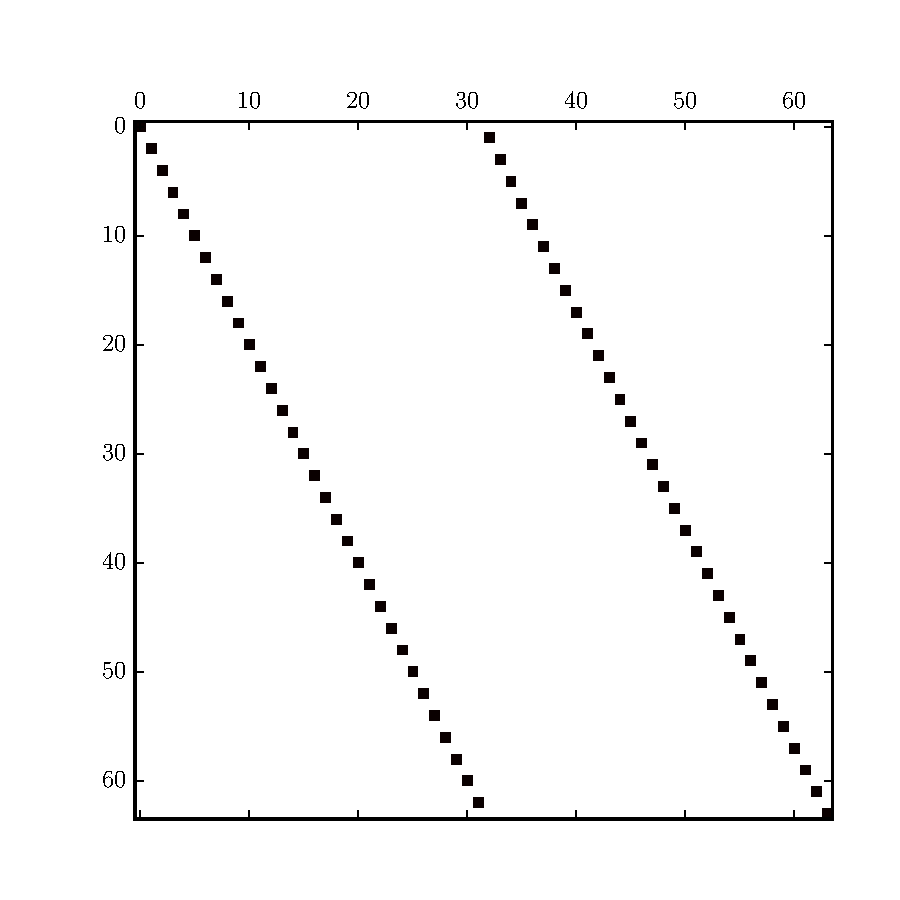
\includegraphics[trim={1cm 1.2cm 1.0cm 1cm},clip,width=0.4\textwidth]{../../figures/perm_mtrx.pdf}
    % %     \caption{The permutation matrix $\netperm$ acting on $\br{\Hilb^2}^{\otimes 6}$ for the Triangle structure. Black entries represents a value of $1$ and white represents $0$.}
    % %     \label{fig:perm_mtrx}
    % % \end{figure}
    % % Finally, we introduce the a permutation matrix $\netperm$ for the Triangle structure. For bipartite qubit states, $\netperm$ is the $64\times64$ bit-wise matrix depicted in \cref{fig:perm_mtrx}. Upon examination of \cref{eq:quantum_model_triangle_pvms}, we consider $\netperm$ to be acting on the joint global state $\rho_{\p{AB}} \otimes \rho_{\p{BC}} \otimes \rho_{\p{CA}}$. To illuminate its necessity, consider \cref{eq:quantum_model_triangle} in the absence of $\netperm$.
    % % \begin{align*}
    % % \prob[\p{ABC}]\br{abc} &\stackrel{?}{=} \Tr\bs{\br{\rho_{\p{AB}} \otimes \rho_{\p{BC}} \otimes \rho_{\p{CA}}} \br{M^a_{\p{A}}\otimes M^b_{\p{B}} \otimes M^c_{\p{C}}}}\\
    % % &= \Tr\bs{\br{\rho_{\p{AB}}M^a_{\p{A}}}\otimes\br{\rho_{\p{BC}}M^b_{\p{B}}}\otimes\br{\rho_{\p{CA}}M^c_{\p{C}}}}\\
    % % &= \Tr\br{\rho_{\p{AB}}M^a_{\p{A}}}\Tr\br{\rho_{\p{BC}}M^b_{\p{B}}}\Tr\br{\rho_{\p{CA}}M^c_{\p{C}}}\\
    % % &= \prob[\p{A}\mid \rho_{\p{AB}}]\br{a}\prob[\p{B}\mid \rho_{\p{BC}}]\br{b}\prob[\p{C}\mid \rho_{\p{CA}}]\br{c}
    % % \end{align*}
    % % On an operational level, this corresponds to $A$ making a measurement on \textit{both} subsystems of $\rho_{AB}$ and \textit{not} on any component of $\rho_{CA}$. This is analogously troubling for $B$ and $C$ as well. To resolve this issue, the permutation matrix $\netperm$ corresponds to \textit{aligning} the underlying $6$-qubit joint state $\rho$ with the joint measurement $M$. To understand its effect, consider its effect on $6$-qubit pure state $\ket{q_1} \otimes \cdots \otimes \ket{q_6} = \ket{q_1q_2q_3q_4q_5q_6}$ where $\forall i : \ket{q_i} \in \Hilb^2$.
    % % \[ \netperm\ket{q_1q_2q_3q_4q_5q_6} = \ket{q_2q_3q_4q_5q_6q_1} \]
    % % $\netperm$ acts as a \textit{partial transpose} on $\br{\Hilb^2}^{\otimes 6}$ by shifting the underlying tensor structure one subsystem to the ``left''. It is uniquely defined by its action on all $2^6$ orthonormal basis elements of $\br{\Hilb^2}^{\otimes 6}$,
    % % \[ \netperm \defined \sum_{\ket{q_i} \in \bc{\ket{0}, \ket{1}}}\ket{q_2q_3q_4q_5q_6q_1}\bra{q_1q_2q_3q_4q_5q_6} \]
    % \subsection{Computationally Efficient Parameterization of the Unitary Group}
    % \label{sec:comp_spengler}

    % If \cref{sec:unitary_group}, the SSH parameterization was introduced as a non-degenerate parameterization of the unitary group $\s{U}\br{d}$. As presented, the SSH parameterization suffers due to the presence of computationally expensive matrix exponential terms~\cite{Moler_2003}. Although not explicitly mentioned in~\cite{Spengler_2010_Unitary}, it is possible to remove the reliance on matrix exponential operations in \cref{eq:spengler_unitary} by utilizing the explicit form of the exponential terms in \cref{eq:exp_terms}. As a first step, recognize the defining property of the projective operators \cref{eq:projective_operator},
    % \[ P_l^k = \br{\ket{l}\bra{l}}^k = \ket{l}\bra{l} = P_l \]
    % This greatly simplifies the global phase terms $GP_l$,
    % \[ GP_l = \exp\br{iP_l \lambda_{l,l}} = \sum_{k=0}^{\inf} \f{\br{iP_l \lambda_{l,l}}^k}{k!} = \ident + \sum_{k=1}^{\inf} \f{\br{i \lambda_{l,l}}^k}{k!}P_l^k = \ident + P_l \bs{\sum_{k=1}^{\inf} \f{\br{i \lambda_{l,l}}^k}{k!}} = \ident + P_l \br{e^{i \lambda_{l,l}} - 1} \eq \label{eq:unitary_GP} \]
    % Analogously for the relative phase terms $RP_{n,m}$,
    % \[ RP_{n,m} = \cdots = \ident + P_n \br{e^{i \lambda_{n,m}} - 1} \eq \label{eq:unitary_RP} \]
    % Finally, the rotation terms $R_{m,n}$ can also be simplified by examining powers of $i \sigma_{n,m}$,
    % \[ R_{m,n} = \exp\br{i \si_{m,n} \lambda_{m,n}} = \sum_{k=0}^{\inf} \f{\br{\ket{m}\bra{n} - \ket{n}\bra{m}}^k \lambda_{m,n}^k}{k!} \]
    % One can verify that the following properties hold,
    % \begin{align*}
    %     \br{\ket{m}\bra{n} - \ket{n}\bra{m}}^0 &= \ident \\
    %     \forall k \in \N, k \neq 0 : \br{\ket{m}\bra{n} - \ket{n}\bra{m}}^{2k} &= \br{-1}^k\br{\ket{m}\bra{m} + \ket{n}\bra{n}} \\
    %     \forall k \in \N : \br{\ket{m}\bra{n} - \ket{n}\bra{m}}^{2k+1} &= \br{-1}^k\br{\ket{m}\bra{n} - \ket{n}\bra{m}}
    % \end{align*}
    % Revealing the simplified form of $R_{m,n}$,
    % \[ R_{m,n} = \ident + \br{\ket{m}\bra{m} + \ket{n}\bra{n}} \sum_{j=1}^{\inf} \br{-1}^j\f{\lambda_{n,m}^{2j}}{\br{2j}!} + \br{\ket{m}\bra{n} - \ket{n}\bra{m}} \sum_{j=0}^{\inf} \br{-1}^j\f{\lambda_{n,m}^{2j+1}}{\br{2j+1}!} \]
    % \[ R_{m,n} = \ident + \br{\ket{m}\bra{m} + \ket{n}\bra{n}} \br{\cos\lambda_{n,m} - 1} + \br{\ket{m}\bra{n} - \ket{n}\bra{m}} \sin\lambda_{n,m} \eq \label{eq:unitary_R} \]
    % By combining the optimizations of \cref{eq:unitary_GP,eq:unitary_RP,eq:unitary_R} together we arrive at an equivalent form for \cref{eq:spengler_unitary} that is computational more efficient.
    % \[ U = \bs{\prod_{m=1}^{d-1} \br{\prod_{n=m+1}^{d} R_{m,n}RP_{n,m}}} \cdot \bs{\prod_{l=1}^{d} GP_{l}}  \eq \label{eq:spengler_unitary_fast} \]

    \setlength{\bibsep}{3pt plus 3pt minus 2pt}
    \bibliographystyle{apsrev4-1}
    % \nocite{apsrev41Control}
    \bibliography{references}

\end{document}